
%% bare_conf.tex
%% V1.4b
%% 2015/08/26
%% by Michael Shell
%% See:
%% http://www.michaelshell.org/
%% for current contact information.
%%
%% This is a skeleton file demonstrating the use of IEEEtran.cls
%% (requires IEEEtran.cls version 1.8b or later) with an IEEE
%% conference paper.
%%
%% Support sites:
%% http://www.michaelshell.org/tex/ieeetran/
%% http://www.ctan.org/pkg/ieeetran
%% and
%% http://www.ieee.org/

%%*************************************************************************
%% Legal Notice:
%% This code is offered as-is without any warranty either expressed or
%% implied; without even the implied warranty of MERCHANTABILITY or
%% FITNESS FOR A PARTICULAR PURPOSE! 
%% User assumes all risk.
%% In no event shall the IEEE or any contributor to this code be liable for
%% any damages or losses, including, but not limited to, incidental,
%% consequential, or any other damages, resulting from the use or misuse
%% of any information contained here.
%%
%% All comments are the opinions of their respective authors and are not
%% necessarily endorsed by the IEEE.
%%
%% This work is distributed under the LaTeX Project Public License (LPPL)
%% ( http://www.latex-project.org/ ) version 1.3, and may be freely used,
%% distributed and modified. A copy of the LPPL, version 1.3, is included
%% in the base LaTeX documentation of all distributions of LaTeX released
%% 2003/12/01 or later.
%% Retain all contribution notices and credits.
%% ** Modified files should be clearly indicated as such, including  **
%% ** renaming them and changing author support contact information. **
%%*************************************************************************


% *** Authors should verify (and, if needed, correct) their LaTeX system  ***
% *** with the testflow diagnostic prior to trusting their LaTeX platform ***
% *** with production work. The IEEE's font choices and paper sizes can   ***
% *** trigger bugs that do not appear when using other class files.       ***                          ***
% The testflow support page is at:
% http://www.michaelshell.org/tex/testflow/



\documentclass[journal]{IEEEtran}
% Some Computer Society conferences also require the compsoc mode option,
% but others use the standard conference format.
%
% If IEEEtran.cls has not been installed into the LaTeX system files,
% manually specify the path to it like:
% \documentclass[conference]{../sty/IEEEtran}


% Some very useful LaTeX packages include:
% (uncomment the ones you want to load)


% *** MISC UTILITY PACKAGES ***
%
%\usepackage{ifpdf}
% Heiko Oberdiek's ifpdf.sty is very useful if you need conditional
% compilation based on whether the output is pdf or dvi.
% usage:
% \ifpdf
%   % pdf code
% \else
%   % dvi code
% \fi
% The latest version of ifpdf.sty can be obtained from:
% http://www.ctan.org/pkg/ifpdf
% Also, note that IEEEtran.cls V1.7 and later provides a builtin
% \ifCLASSINFOpdf conditional that works the same way.
% When switching from latex to pdflatex and vice-versa, the compiler may
% have to be run twice to clear warning/error messages.



% *** CITATION PACKAGES ***
%
%\usepackage{cite}
% cite.sty was written by Donald Arseneau
% V1.6 and later of IEEEtran pre-defines the format of the cite.sty package
% \cite{} output to follow that of the IEEE. Loading the cite package will
% result in citation numbers being automatically sorted and properly
% "compressed/ranged". e.g., [1], [9], [2], [7], [5], [6] without using
% cite.sty will become [1], [2], [5]--[7], [9] using cite.sty. cite.sty's
% \cite will automatically add leading space, if needed. Use cite.sty's
% noadjust option (cite.sty V3.8 and later) if you want to turn this off
% such as if a citation ever needs to be enclosed in parenthesis.
% cite.sty is already installed on most LaTeX systems. Be sure and use
% version 5.0 (2009-03-20) and later if using hyperref.sty.
% The latest version can be obtained at:
% http://www.ctan.org/pkg/cite
% The documentation is contained in the cite.sty file itself.






% *** GRAPHICS RELATED PACKAGES ***
%
\ifCLASSINFOpdf
  % \usepackage[pdftex]{graphicx}
  % declare the path(s) where your graphic files are
  % \graphicspath{{../pdf/}{../jpeg/}}
  % and their extensions so you won't have to specify these with
  % every instance of \includegraphics
  % \DeclareGraphicsExtensions{.pdf,.jpeg,.png}
\else
  % or other class option (dvipsone, dvipdf, if not using dvips). graphicx
  % will default to the driver specified in the system graphics.cfg if no
  % driver is specified.
  % \usepackage[dvips]{graphicx}
  % declare the path(s) where your graphic files are
  % \graphicspath{{../eps/}}
  % and their extensions so you won't have to specify these with
  % every instance of \includegraphics
  % \DeclareGraphicsExtensions{.eps}
\fi
% graphicx was written by David Carlisle and Sebastian Rahtz. It is
% required if you want graphics, photos, etc. graphicx.sty is already
% installed on most LaTeX systems. The latest version and documentation
% can be obtained at: 
% http://www.ctan.org/pkg/graphicx
% Another good source of documentation is "Using Imported Graphics in
% LaTeX2e" by Keith Reckdahl which can be found at:
% http://www.ctan.org/pkg/epslatex
%
% latex, and pdflatex in dvi mode, support graphics in encapsulated
% postscript (.eps) format. pdflatex in pdf mode supports graphics
% in .pdf, .jpeg, .png and .mps (metapost) formats. Users should ensure
% that all non-photo figures use a vector format (.eps, .pdf, .mps) and
% not a bitmapped formats (.jpeg, .png). The IEEE frowns on bitmapped formats
% which can result in "jaggedy"/blurry rendering of lines and letters as
% well as large increases in file sizes.
%
% You can find documentation about the pdfTeX application at:
% http://www.tug.org/applications/pdftex





% *** MATH PACKAGES ***
%
%\usepackage{amsmath}
% A popular package from the American Mathematical Society that provides
% many useful and powerful commands for dealing with mathematics.
%
% Note that the amsmath package sets \interdisplaylinepenalty to 10000
% thus preventing page breaks from occurring within multiline equations. Use:
%\interdisplaylinepenalty=2500
% after loading amsmath to restore such page breaks as IEEEtran.cls normally
% does. amsmath.sty is already installed on most LaTeX systems. The latest
% version and documentation can be obtained at:
% http://www.ctan.org/pkg/amsmath





% *** SPECIALIZED LIST PACKAGES ***
%
% \usepackage{algorithmic}
% algorithmic.sty was written by Peter Williams and Rogerio Brito.
% This package provides an algorithmic environment fo describing algorithms.
% You can use the algorithmic environment in-text or within a figure
% environment to provide for a floating algorithm. Do NOT use the algorithm
% floating environment provided by algorithm.sty (by the same authors) or
% algorithm2e.sty (by Christophe Fiorio) as the IEEE does not use dedicated
% algorithm float types and packages that provide these will not provide
% correct IEEE style captions. The latest version and documentation of
% algorithmic.sty can be obtained at:
% http://www.ctan.org/pkg/algorithms
% Also of interest may be the (relatively newer and more customizable)
% algorithmicx.sty package by Szasz Janos:
% http://www.ctan.org/pkg/algorithmicx




% *** ALIGNMENT PACKAGES ***
%
%\usepackage{array}
% Frank Mittelbach's and David Carlisle's array.sty patches and improves
% the standard LaTeX2e array and tabular environments to provide better
% appearance and additional user controls. As the default LaTeX2e table
% generation code is lacking to the point of almost being broken with
% respect to the quality of the end results, all users are strongly
% advised to use an enhanced (at the very least that provided by array.sty)
% set of table tools. array.sty is already installed on most systems. The
% latest version and documentation can be obtained at:
% http://www.ctan.org/pkg/array


%% IEEEtran contains the IEEEarray family of commands that can be used to
% generate multiline equations as well as matrices, tables, etc., of high
% quality.

% *** SUBFIGURE PACKAGES ***
%\ifCLASSOPTIONcompsoc
%  \usepackage[caption=false,font=normalsize,labelfont=sf,textfont=sf]{subfig}
%\else
%  \usepackage[caption=false,font=footnotesize]{subfig}
%\fi
% subfig.sty, written by Steven Douglas Cochran, is the modern replacement
% for subfigure.sty, the latter of which is no longer maintained and is
% incompatible with some LaTeX packages including fixltx2e. However,
% subfig.sty requires and automatically loads Axel Sommerfeldt's caption.sty
% which will override IEEEtran.cls' handling of captions and this will result
% in non-IEEE style figure/table captions. To prevent this problem, be sure
% and invoke subfig.sty's "caption=false" package option (available since
% subfig.sty version 1.3, 2005/06/28) as this is will preserve IEEEtran.cls
% handling of captions.
% Note that the Computer Society format requires a larger sans serif font
% than the serif footnote size font used in traditional IEEE formatting
% and thus the need to invoke different subfig.sty package options depending
% on whether compsoc mode has been enabled.
%
% The latest version and documentation of subfig.sty can be obtained at:
% http://www.ctan.org/pkg/subfig




% *** FLOAT PACKAGES ***
%
%\usepackage{fixltx2e}
% fixltx2e, the successor to the earlier fix2col.sty, was written by
% Frank Mittelbach and David Carlisle. This package corrects a few problems
% in the LaTeX2e kernel, the most notable of which is that in current
% LaTeX2e releases, the ordering of single and double column floats is not
% guaranteed to be preserved. Thus, an unpatched LaTeX2e can allow a
% single column figure to be placed prior to an earlier double column
% figure.
% Be aware that LaTeX2e kernels dated 2015 and later have fixltx2e.sty's
% corrections already built into the system in which case a warning will
% be issued if an attempt is made to load fixltx2e.sty as it is no longer
% needed.
% The latest version and documentation can be found at:
% http://www.ctan.org/pkg/fixltx2e


%\usepackage{stfloats}
% stfloats.sty was written by Sigitas Tolusis. This package gives LaTeX2e
% the ability to do double column floats at the bottom of the page as well
% as the top. (e.g., "\begin{figure*}[!b]" is not normally possible in
% LaTeX2e). It also provides a command:
%\fnbelowfloat
% to enable the placement of footnotes below bottom floats (the standard
% LaTeX2e kernel puts them above bottom floats). This is an invasive package
% which rewrites many portions of the LaTeX2e float routines. It may not work
% with other packages that modify the LaTeX2e float routines. The latest
% version and documentation can be obtained at:
% http://www.ctan.org/pkg/stfloats
% Do not use the stfloats baselinefloat ability as the IEEE does not allow
% \baselineskip to stretch. Authors submitting work to the IEEE should note
% that the IEEE rarely uses double column equations and that authors should try
% to avoid such use. Do not be tempted to use the cuted.sty or midfloat.sty
% packages (also by Sigitas Tolusis) as the IEEE does not format its papers in
% such ways.
% Do not attempt to use stfloats with fixltx2e as they are incompatible.
% Instead, use Morten Hogholm'a dblfloatfix which combines the features
% of both fixltx2e and stfloats:
%
% \usepackage{dblfloatfix}
% The latest version can be found at:
% http://www.ctan.org/pkg/dblfloatfix




% *** PDF, URL AND HYPERLINK PACKAGES ***
%
%\usepackage{url}
% url.sty was written by Donald Arseneau. It provides better support for
% handling and breaking URLs. url.sty is already installed on most LaTeX
% systems. The latest version and documentation can be obtained at:
% http://www.ctan.org/pkg/url
% Basically, \url{my_url_here}.




% *** Do not adjust lengths that control margins, column widths, etc. ***
% *** Do not use packages that alter fonts (such as pslatex).         ***
% There should be no need to do such things with IEEEtran.cls V1.6 and later.
% (Unless specifically asked to do so by the journal or conference you plan
% to submit to, of course. )

% *** packages included here ***
\usepackage{algorithm}
\usepackage{algorithmic}
%\usepackage{algpseudocode}
\usepackage{graphicx}
\usepackage{amsmath}
\usepackage{amsthm}
\usepackage{multirow}
\usepackage{balance}
\usepackage{xspace}
\usepackage{amssymb}

% *** Let's defined our own macros here ***
\newcommand{\calG}{\mathcal{G}}
\newcommand{\calV}{\mathcal{V}}
\newcommand{\calL}{\mathcal{L}}
\newcommand{\calS}{\mathcal{S}}
\newcommand{\calR}{\mathcal{R}}
\newcommand{\calD}{\mathcal{D}}
\newcommand{\calT}{\mathcal{T}}
\newcommand{\calH}{\mathcal{H}}
\newcommand{\width}{\mathit{W}_\calG}
\newcommand{\SD}{\mathit{SD}_\calG}
\newcommand{\HD}{\mathit{LD}_\calG}
\newcommand{\MT}{\mathit{MT}_\calG}
\newcommand{\route}[3]{#1^{\langle #2,#3\rangle}}

\theoremstyle{remark}
\newtheorem{constraint}{Constraint}
%\newtheorem{lemma}[theorem]{Lemma}
%\newtheorem{definition}[theorem]{Definition}

% for comments
\newcommand{\jx}[1]{\%\% \textbf{Jiaxixang: }#1 \%\%\xspace}
%\renewcommand{\jx}[1]{\ignorespaces}

% correct bad hyphenation here
\hyphenation{op-tical net-works semi-conduc-tor}


\begin{document}
%
% paper title
% Titles are generally capitalized except for words such as a, an, and, as,
% at, but, by, for, in, nor, of, on, or, the, to and up, which are usually
% not capitalized unless they are the first or last word of the title.
% Linebreaks \\ can be used within to get better formatting as desired.
% Do not put math or special symbols in the title.
\title{Effective Static Scheduling of a Time-Triggered Network-on-Chip with Memetic Algorithm}


% author names and affiliations
% use a multiple column layout for up to three different
% affiliations



\author{
	\IEEEauthorblockN{
		Heyuan Shi\\
		}
	\IEEEauthorblockA{
		School of Software\\
		Tsinghua University\\
		Beijing, China\\
		Email: shy15@tsinghua.edu.cn}
}



%\author{
%	\IEEEauthorblockN{Heyuan Shi}
%	\IEEEauthorblockA{
%		School of Software\\
%		Tsinghua University\\
%		Beijing, China\\
%		Email: hey.shi@foxmail.com}
%



% conference papers do not typically use \thanks and this command
% is locked out in conference mode. If really needed, such as for
% the acknowledgment of grants, issue a \IEEEoverridecommandlockouts
% after \documentclass

% for over three affiliations, or if they all won't fit within the width
% of the page, use this alternative format:
% 
%\author{\IEEEauthorblockN{Michael Shell\IEEEauthorrefmark{1},
%Homer Simpson\IEEEauthorrefmark{2},
%James Kirk\IEEEauthorrefmark{3}, 
%Montgomery Scott\IEEEauthorrefmark{3} and
%Eldon Tyrell\IEEEauthorrefmark{4}}
%\IEEEauthorblockA{\IEEEauthorrefmark{1}School of Electrical and Computer Engineering\\
%Georgia Institute of Technology,
%Atlanta, Georgia 30332--0250\\ Email: see http://www.michaelshell.org/contact.html}
%\IEEEauthorblockA{\IEEEauthorrefmark{2}Twentieth Century Fox, Springfield, USA\\
%Email: homer@thesimpsons.com}
%\IEEEauthorblockA{\IEEEauthorrefmark{3}Starfleet Academy, San Francisco, California 96678-2391\\
%Telephone: (800) 555--1212, Fax: (888) 555--1212}
%\IEEEauthorblockA{\IEEEauthorrefmark{4}Tyrell Inc., 123 Replicant Street, Los Angeles, California 90210--4321}}




% use for special paper notices
%\IEEEspecialpapernotice{(Invited Paper)}




% make the title area
\maketitle

% As a general rule, do not put math, special symbols or citations
% in the abstract
\begin{abstract}
	
Time-Triggered Network-on-Chip (TTNoC) is a time-triggered embedded system deployed on the Network-on-Chip (NoC). 
It ensures the reliable and safety-critical industrial communication for real-time embedded multiprocessor systems. 
To guarantee the safe-critical requirements for communication, each message is transmitted by a predefined static schedule. 
However,
 synthesizing the scheduling is a challenging problem because both path contention and the temporal constraints should be considered. 
To resolve this problem, this paper presents a novel memetic algorithm (MA) which incorporates local search in the genetic algorithm. 
For given architecture of TTNoC and messages for communication,
the offset for messages is synthesized by MA, ensuring no contention with the communications on the TTNoC.
We compare our memetic algorithm with the general genetic algorithm.
The experimental results show that
the failed scheduling of MA is 
only about 30\% percent in average of that of the conventional genetic algorithm.
\end{abstract}
% no keywords

% For peer review papers, you can put extra information on the cover
% page as needed:
% \ifCLASSOPTIONpeerreview
% \begin{center} \bfseries EDICS Category: 3-BBND \end{center}
% \fi
%
% For peerreview papers, this IEEEtran command inserts a page break and
% creates the second title. It will be ignored for other modes.
\IEEEpeerreviewmaketitle



\section{Introduction}

Time-triggered systems is one of the real-time systems with high throughput and temporal predictability for industrial multiprocessor systems~\cite{DBLP:journals/rts/CraciunasO16}.
Time-triggered systems isolating the inherent faults as well as satisfying the temporal predictability of communication and widely deployed in various field, e.g.
TTEthernet integrates time-triggered concept into the general Ethernet~\cite{DBLP:conf/nca/SteinerBHPV09}, which is adopted as a new standard of the avionic network~\cite{DBLP:conf/dsrt/BejiHGM14}. TTP and FlexRay are adopted in aerospace industry~\cite{DBLP:journals/taes/HuLWV15}.

TTNoC integrates the time-triggered concepts into the Network-on-Chip (NoC) for safety-critical real-time embedded systems, which requires the tight and predictable communication latency.
In practice,
 GENESYS is proposed as a cross-domain embedded system architecture,
  which influenced by the concepts of and the experience with the time-triggered architecture~\cite{DBLP:conf/ladc/Kopetz11}.

There are two main architectures of a time-triggered system,
 bus-based and network-based architecture~\cite{DBLP:conf/date/HuangBRBK12}.
There is only one message transmitted on the system at the same time in the bus-based architecture. 
Therefore, each message owns its unique duration to communicate through the physical link.
Unlike the bus-based architecture,
 the network-based architecture allows a set of messages to be transmitted at the same time,
  provided that the physical links used by the messages are non-overlapping.
It entails messages sharing the time domain to communicate.
Fig.~\ref{f:diff} shows the differences between bus-based and network-based time-triggered architectures.
In a bus-based architecture,
 all the messages ($\tau_0$,$\tau_1$,$\tau_2$) achieve temporal separation. 
In a network-based architecture,
 the set of messages ($\tau_0$,$\tau_1$,$\tau_2$) can share the time domain if there is no spatial conflict among the transmission of them.
\begin{figure}[!t]
	\centering
	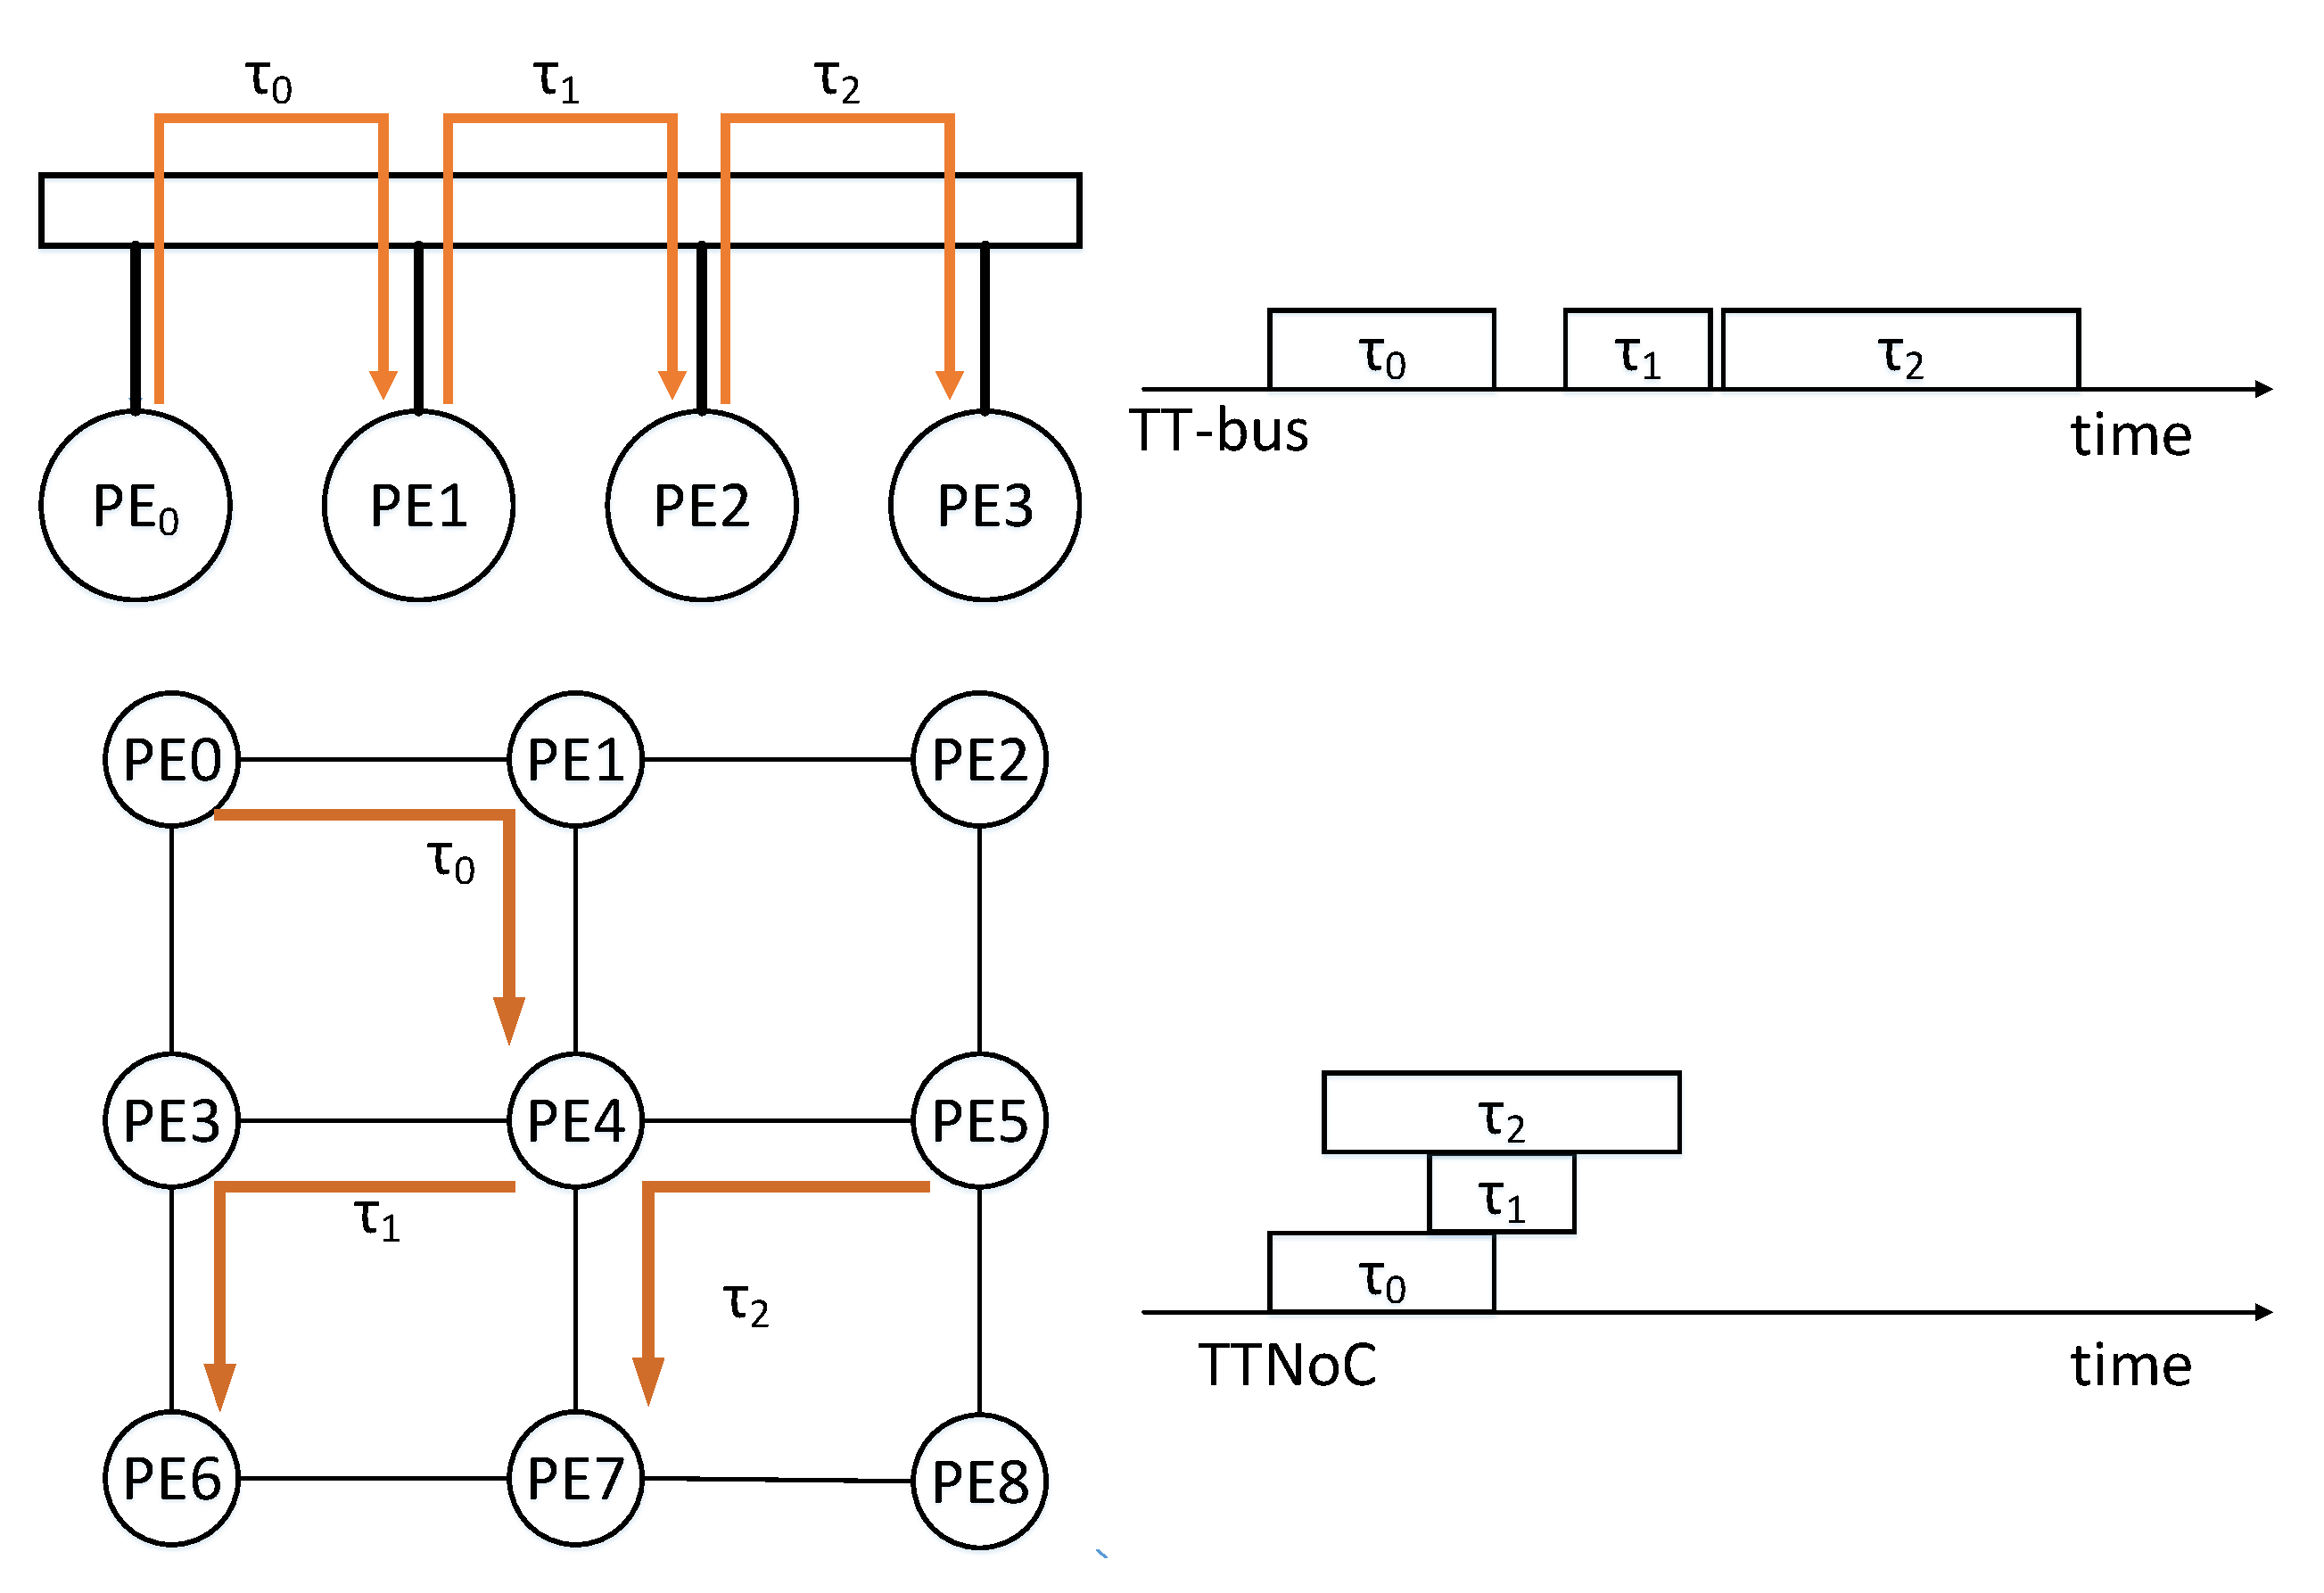
\includegraphics[width=3in]{picture/difference.pdf}
	\caption{Difference between bus- and network-based time-triggered architecture}
	\label{f:diff}
\end{figure}

A TTNoC employs the network-based architecture.
The scheduling of TTNoC is to determine the duration of each message and ensure that there is no contentions on the TTNoC. 
Static scheduling is adopted to synthesize the scheduling which resolves contention,
thus avoiding dynamic arbitration of intercommunicate resources distribution. 
Hence, the communication on the TTNoC is predefined while satisfying the scheduling constraints.
However,
 synthesizing such a scheduling is rather complicated which is known as NP-complete problem~\cite{DBLP:conf/date/HuangBRBK12,DBLP:conf/rtss/Steiner10}.

The main contribution of this paper is a static scheduling approach to resolve the TTNoC scheduling problem by a memetic algorithm. 
MA is widely used as a synergy of evolutionary or any population-based approach with separate individual learning or local improvement procedures for solution search~\cite{DBLP:journals/tec/ChenOLT11}. 

The rest of this paper is organized as follows. 
We first review the related work in the TTNoC scheduling in Section~\ref{s:relate}. 
The system model is given in Section~\ref{s:model},
 followed by the schedule constraints in Section~\ref{s:constraint}.
We presents the problem formulation in Section~\ref{s:formulation}.
A new memetic algorithm is proposed in Section~\ref{s:algorithm}.
The experiments with synthesis results are presented in Section~\ref{s:evalu}.
Finally, we conclude this paper in Section~\ref{s:conclud}.

\section{Related Work	\label{s:relate}}

There are sufficient literatures about the scheduling of time-triggered network,
 which is similar to the scheduling of TTNoC. 
\cite{DBLP:conf/rtss/Steiner10} considers the scheduling of the time-triggered multi-hop networks.
A pure satisfiability modulo theories (SMT) formulation is presented followed by an incremental method to improve the scalability.
\cite{DBLP:journals/rts/CraciunasO16,DBLP:conf/rtns/CraciunasO14} formulate the schedule problem using first-order logical constraints and present alternative methods to find a solution based on SMT and mixed integer programming (MIP) solvers.
In \cite{DBLP:conf/etfa/PozoSRH15} the authors presents a decomposition approach based on SMT solver for extremely large time-triggered network.

The scheduling problem also appear in the various domain.
\cite{DBLP:conf/isorc/RoRM15} resolves the scheduling on the wireless network by SMT solver.
\cite{DBLP:conf/aspdac/ZhangG0C14} formulates the co-synthesis problem of task and communication schedules as a Mixed Integer Programming (MIP) model taking into account a number of Ethernet-specific timing parameters.
Holistic Scheduling in Time-Triggered In-Vehicle Networks was studied in~\cite{DBLP:journals/tii/HuLWLZ14}

The scheduling problem of TTNoC has been
studied firstly in \cite{DBLP:conf/date/HuangBRBK12} which integrates SMT solver into a classical heuristic algorithm. 
\cite{DBLP:conf/sies/ScholerKMO15} presents an optimal scheduler based on a Boolean SAT solver for a TTNoC.
\cite{DBLP:conf/indin/MurshedOAK15} introduces a scheduling model based on Mixed Integer Linear Programming (MILP) combining both time-triggered and event-triggered messages on NoC.
In~\cite{DBLP:conf/sies/FreierC15},
 A heuristic algorithm for scheduling on the scalable communication structure like a NoC is presented. 


% An example of a floating figure using the graphicx package.
% Note that \label must occur AFTER (or within) \caption.
% For figures, \caption should occur after the \includegraphics.
% Note that IEEEtran v1.7 and later has special internal code that
% is designed to preserve the operation of \label within \caption
% even when the captionsoff option is in effect. However, because
% of issues like this, it may be the safest practice to put all your
% \label just after \caption rather than within \caption{}.
%
% Reminder: the "draftcls" or "draftclsnofoot", not "draft", class
% option should be used if it is desired that the figures are to be
% displayed while in draft mode.
%
%\begin{figure}[!t]
%\centering
%\includegraphics[width=2.5in]{myfigure}
% where an .eps filename suffix will be assumed under latex, 
% and a .pdf suffix will be assumed for pdflatex; or what has been declared
% via \DeclareGraphicsExtensions.
%\caption{Simulation results for the network.}
%\label{fig_sim}
%\end{figure}

% Note that the IEEE typically puts floats only at the top, even when this
% results in a large percentage of a column being occupied by floats.


% An example of a double column floating figure using two subfigures.
% (The subfig.sty package must be loaded for this to work.)
% The subfigure \label commands are set within each subfloat command,
% and the \label for the overall figure must come after \caption.
% \hfil is used as a separator to get equal spacing.
% Watch out that the combined width of all the subfigures on a 
% line do not exceed the text width or a line break will occur.
%
%\begin{figure*}[!t]
%\centering
%\subfloat[Case I]{\includegraphics[width=2.5in]{box}%
%\label{fig_first_case}}
%\hfil
%\subfloat[Case II]{\includegraphics[width=2.5in]{box}%
%\label{fig_second_case}}
%\caption{Simulation results for the network.}
%\label{fig_sim}
%\end{figure*}
%
% Note that often IEEE papers with subfigures do not employ subfigure
% captions (using the optional argument to \subfloat[]), but instead will
% reference/describe all of them (a), (b), etc., within the main caption.
% Be aware that for subfig.sty to generate the (a), (b), etc., subfigure
% labels, the optional argument to \subfloat must be present. If a
% subcaption is not desired, just leave its contents blank,
% e.g., \subfloat[].


% An example of a floating table. Note that, for IEEE style tables, the
% \caption command should come BEFORE the table and, given that table
% captions serve much like titles, are usually capitalized except for words
% such as a, an, and, as, at, but, by, for, in, nor, of, on, or, the, to
% and up, which are usually not capitalized unless they are the first or
% last word of the caption. Table text will default to \footnotesize as
% the IEEE normally uses this smaller font for tables.
% The \label must come after \caption as always.
%
%\begin{table}[!t]
%% increase table row spacing, adjust to taste
%\renewcommand{\arraystretch}{1.3}
% if using array.sty, it might be a good idea to tweak the value of
% \extrarowheight as needed to properly center the text within the cells
%\caption{An Example of a Table}
%\label{table_example}
%\centering
%% Some packages, such as MDW tools, offer better commands for making tables
%% than the plain LaTeX2e tabular which is used here.
%\begin{tabular}{|c||c|}
%\hline
%One & Two\\
%\hline
%Three & Four\\
%\hline
%\end{tabular}
%\end{table}


% Note that the IEEE does not put floats in the very first column
% - or typically anywhere on the first page for that matter. Also,
% in-text middle ("here") positioning is typically not used, but it
% is allowed and encouraged for Computer Society conferences (but
% not Computer Society journals). Most IEEE journals/conferences use
% top floats exclusively. 
% Note that, LaTeX2e, unlike IEEE journals/conferences, places
% footnotes above bottom floats. This can be corrected via the
% \fnbelowfloat command of the stfloats package.

\section{System Model}
\label{s:model}

In this section we presents the basis and model of TTNoC.
The system architecture we adopted is shown in~\cite{DBLP:conf/rtcsa/PaukovitsK08}. 

\subsection{Architecture Model}

TTNoC is a system with a set of real-time tasks/applications mapped on a multi-core interconnection platform. 
It composes of a set of identical processing elements (PEs) interconnected by physical links and the switches on the TTNoC.
The switches are connected by bidirectional physical links and each link connects a pair of switches.  
The topologies of a TTNoC can be either regular or irregular.

The architecture of a TTNoC is modeled by a directed graph $\calG=(\calV,\calL)$. 
The set of vertexes $\mathcal{V}=\{ v_{0},\dots,v_{m-1}\}$ represents the set of $m$ \emph{identical} communication nodes (the PEs and switches).
The edges $\mathcal{L}\subseteq \mathcal{V} \times\mathcal{V}$ comprises the communication physical links \emph{directly} connecting the nodes.
The physical links are full-duplex, allowing communication in both directions. 
Therefore, given $v_i,v_j\in\calV$, $\langle v_i,v_j\rangle \in\calL$ implies $\langle v_j,v_i\rangle\in\calL$,
 where $\langle v_i,v_j\rangle$ is a pair denoting a directed physical link connecting two adjacent nodes,
  from a source node $v_i$ to a sink node $v_j$.

Since switches and links are identical on the TTNoC,
 the width of physical links as well as the performance of switches and links is the same,.
The properties of each hop can be regarded as system properties of TTNoC.
Hence a TTNoC $\calG$ is equipped with a set of properties. 
We use $\width$ to denote the width of physical links in the TTNoC,
 $\SD$ for the switching delay in the switches,
  $\HD$ for the link delay per hop which means propagation cost between adjacent nodes,
   and $\MT$ discussed in Section~\ref{ss:schmodel}, for the macrotick of network representing the time-line granularity of the communication on the TTNoC.

%% A network link $(v_{a},v_{b})$, between the source node
%% $v_{a}$ and the sink node $v_{b}$, is defined by the tuple $\langle
%% (v_{a},v_{b}).w, (v_{a},v_{b}).sd,(v_{a},v_{b}).pd,(v_{a},v_{b}).mt,
%% (v_{a},v_{b}).h\rangle$, where $(v_{a},v_{b}).w$ is the width of
%% physical links, $(v_{a},v_{b}).sd$ is the switching delay in the
%% switches on network link, $(v_{a},v_{b}).pd$ is the link delay per hop
%% which means propagation cost between adjacent nodes,
%% $(v_{a},v_{b}).mt$ is the macrotick of network denotes the time-line
%% granularity of the physical link and $(v_{a},v_{b}).h$ is the number
%% of hops from $v_{a}$ to $v_{b}$ on the link $(v_{a},v_{b})$.

Given two nodes $v,v'\in\calV$, a \emph{route} from $v$ to $v'$,
 denoted by $\route{r}{v}{v'}$, is defined as a sequence of the form 
 $\langle v_{k_0},v_{k_1}\rangle\langle
v_{k_1},v_{k_2}\rangle\ldots\langle v_{k_{i-1}},v_{k_i}\rangle\langle
v_{k_i},v_{k_{i+1}}\rangle\ldots \langle v_{k_{n-1}},v_{k_n}\rangle$
satisfying $v_{k_0}=v$, $v_{k_n}=v'$ and $(\forall i\in [1,n])\langle
v_{k_{i-1}},v_{k_i}\rangle \in\calL$. The length $n$ of the route is
written as $|\route{r}{v}{v'}|$. A route $\route{r}{v_i}{v_j}$
represents a \emph{possibly indirect} physical link from $v_i$ to
$v_j$ in the TTNoC, hence its length $|\route{r}{v_i}{v_j}|$ is the
number of hops along this link.

%% For a communication node $ \mathit{v}_{i}\in\mathcal{V} $, it offer
%% $\mathit{d}$ input links and $\mathit{d}$ output links, $\mathit{d}$
%% is the switch degree. Therefore a switch is able to connected with at
%% most $ \mathit{d} $ port in full-duplex connection. The adjoint
%% switches $v_{i}\in\mathcal{V}$ and $v_{j}\in\mathcal{V}$ which connect
%% with each other through physical link rather than the forwarding by
%% other switches, is defined by the sequence $ <v_{i},v_{j}>
%% $. Therefore the network link $(v_{a},v_{b})$ can be split in several
%% connection among the adjoint switches $v_{i}\in\mathcal{V}$, and we
%% have that $ (v_{a},v_{b})=\{ \langle v_{a},v_{1}> ,\dots,
%% <v_{i},v_{j}> ,\dots, <v_{n},v_{b}> \} $.  


\subsection{Message Model}

The communication on the TTNoC is based on messages.  
A message consists of header and data.  
Header includes the information for message forwarding on the TTNoC,
 e.g. the addresses of source and destination. 
Flit is the unit of a message that can be transmitted over the TTNoC.  
Only periodic messages are discussed in this paper because it is the typical case in real-time embedded systems.

We denote the set of $n$ time-triggered messages on the TTNoC by $\Gamma = \{\tau_{0},\dots,\tau_{n-1}\}$. 
Each message $\tau_{i}$ is modeled by the tuple $\langle \tau_{i}.H,\tau_{i}.S, \tau_{i}.T,\tau_{i}.D\rangle$, 
 where $\tau_{i}.H$ denotes the header of the message in flits,
 $\tau_{i}.S$ denotes the size of the message in flits, 
 $\tau_{i}.T$ and $\tau_{i}.D$ are the period and the relative deadline of the message, respectively.
 
\subsection{Scheduling Model}
\label{ss:schmodel}

When the communication happens on the TTNoC between two nodes,
 e.g. a source node $v_i\in \calV$ sends a message $\tau_{k}$ to a sink node $v_j\in \calV$ on the TTNoC,
  the message $\tau_k$ is transmitted on some route $\route{r_k}{v_i}{v_j}$. 
The communication nodes forward the message based on the route $\route{r_k}{v_i}{v_j}$ .

The TDMA scheme is deployed for the scheduling of communication .  
And the time granularity is \emph{macrotick} that the period and relative deadline of message directly match to this time format.

Based on the architecture and message model,
 we can model the scheduling of communication as a set $\calS=\{s_1,\ldots,s_n\}$,
  in which each $s_{i}$ denotes the communication scheduling of the message $\tau_{i}\in\Gamma$. 
Each scheduling $s_{i}\in\calS$ is defined by a tuple $\langle s_i.R, s_i.\phi, s_i.T, s_i.D, s_i.L\rangle$,
 where $s_i.R$ is the route along which the message $\tau_i$ is forwarded, 
 $s_i.\phi$ is the offset of the message,
  $s_i.T$ and
   $s_i.D$ denote the period and the relative deadline of the message in macrotick respectively,
    and $s_i.L$ is the communication delay in macrotick.

For the whole scheduling set $\calS$,
 the sets of the route,
  the period,
   the relative deadline and the delay of each $s_i\in\calS$ are defined as expected,
 denoted by $\calS.\calR$,
  $\calS.\Phi$,
   $\calS.\calT$,
    $\calS.\calD$ and $\calS.\calL$,
     respectively.

%% Based on the architecture and message model, we can model the set of
%% message communication $\mathcal{M}=\{ s_{1},\dots,s_{i}\}$, where
%% $s_{i}\in\mathcal{M}$ denotes the communication scheduling of a
%% message $\tau_{i}\in\Gamma$. For each message $\tau_{i}\in\Gamma$ on
%% the link $(v_{a},v_{b}) $ where $v_{a},v_{b}\in\mathcal{V}$, we model
%% the communication $s_{i}\in\mathcal{M}$ as a tuple $\langle
%% s_{i}^{(v_{a},v_{b})}.\phi, s_{i}^{(v_{a},v_{b})}.\mathcal{T},
%% s_{i}^{(v_{a},v_{b})}.\mathcal{D},s_{i}^{(v_{a},v_{b})}.\mathcal{L}
%% \rangle$, where $ s_{i}^{(v_{a},v_{b})}.\phi$ is the offset of
%% communication, $ s_{i}^{(v_{a},v_{b})}.\mathcal{T} $ is the period of
%% communication, $s_{i}^{(v_{a},v_{b})}.\mathcal{D}$ is the relative
%% deadline of communication, $s_{i}^{(v_{a},v_{b})}.\mathcal{L}$ is the
%% duration of communication and $(v_{a},v_{b})$ in the tuple is the
%% network link for communication.

Because of the macrotick as the granularity of communication,
 for each communication $s_{i}$,
   we have the following formulas:
\begin{equation}
\label{e:eqn1}
  s_i.T = \lceil\frac{\tau_{i}.T}{\MT} \rceil
\end{equation}
\begin{equation}
\label{e:eqn2}
  s_i.D = \lceil\frac{\tau_{i}.D}{\MT}\rceil
\end{equation}
\begin{equation}
\label{e:eqn3}
  s_i.L = \lceil\frac{|s_i.R| \times (\SD+\HD) \times
    \lceil\frac{\tau_{i}.S + \tau_{i}.H}{\tau_{i}.H  }\rceil}{\MT}\rceil
%\lceil\frac{\tau_{i}.s\times (v_{a},v_{b}).sc+(v_{a},v_{b}).delay}{ (v_{a},v_{b}).mt}\rceil 
\end{equation}   
%% where $(v_{a},v_{b}).d = (v_{a},v_{b}).sd+(v_{a},v_{b}).pd $ denotes
%% the delay of propagating and switching delay per hop.
where $\MT$ denotes the value of macrotick,
 and $\SD+\HD$ is the delay per hop in the forwarding.
%% that $\SD$ is the delay on the physical link and $\HD$is the switching delay.

The formula is based on~\cite{DBLP:books/daglib/0087651} with the
modification of adopting macrotick as the unit.  Given an
$s_{i}\in\calS$ and its route $s_i.R$, $s_i.T$, $s_i.D$ and $s_i.L$
can be derived by formulas~\ref{e:eqn1}, \ref{e:eqn2}
and~\ref{e:eqn3}.  Formulas~\ref{e:eqn1} and~\ref{e:eqn2} denote,
respectively, the period and the deadline of the communication $s_i$
in macrotick.  Formula~\ref{e:eqn3} computes the time cost in
macrotick, from the first flit sent by the source node to the last
flit received by the sink node, according to the store-and-forward
(SAF) switching scheme~\cite{DBLP:books/daglib/0087651}.  Moreover,
other scheme of switching on the NoC can be also deployed in the TTNoC
according to the requirements. In this case, the delay Formula
\ref{e:eqn3} should be changed according to the given switching
scheme.

As a result, to synthesize the set of communication $\calS$ is to
calculate the offset $s_i.\phi$ for each communication
$s_i\in\calS$. Therefore, the key to scheduling of TTNoC is to derive
$\calS.\Phi = \{s_i.\phi\mid s_i\in\calS\}$ based on the given
architecture model $\calG$ and the messages model $\Gamma$ with
\emph{scheduling constraints}.


\section{Scheduling Constraints\label{s:constraint}}

The scheduling constraints for general time-triggered multi-hop
network are presented in~\cite{DBLP:conf/rtss/Steiner10}. The
scheduling constraints on TTNoC are similar with those on general
time-triggered network, while some differences exist in terms of our
model.

The synthesized scheduling must satisfy the separation
of the messages in time domain or space domain.
Scheduling of communication $\calS$ should resolve the constraints on
the TTNoC, which mainly including offset constraints and link constraints.

In our TTNoC, scheme of bufferless NoCs is adopted that no buffering
of messages takes place. It leads to significantly less area and
power consumption for TTNoC~\cite{DBLP:journals/tpds/ShpinerKLCK15}.
The route of each message is located on its header.  
The switches simply forward the message according to the address of next-hop
switch, without concerning the communication schedule~\cite{DBLP:conf/rtcsa/PaukovitsK08}. Therefore,
unlike the general time-triggered network, the switch memory
constraints are not concerned. Moreover for
the simplicity of evaluation,
the simultaneous relay,
application-level, protocol-based and domain-specific constraints are neither
concerned.

\subsection{Message Offset Constraints}
For each scheduling of message $s_{i}\in\calS$ , the offset $s_i.\phi$
must be non-negative values and should guarantee that the message
transmission is completed before the deadline of the
communication. Therefore we have that
%\begin{equation}
\begin{constraint}
\label{c:offset}
$(s_i.\phi \geq 0) \cap (s_i.\phi + s_i.L \leq s_i.D)$.
%\end{equation}
\end{constraint}

\subsection{Link Contention Constraints}
For each communication, the message occupies the link in terms of
routing strategy without contention, until the whole message is
received by the sink node. The scheduling $\calS$ should ensure that
two messages are never transmitted on the identical link at the same
time. The synthesized scheduling must guarantee that the links on
TTNoC are contention-free.

Given two scheduling of messages $s_i,s_j\in\calS$,
%$s_{i},s_{j}\in\mathcal{M}, s_{i}\neq s_{j}$,
we define $overlap(s_i,s_j)$ to indicate whether there are any common
physical links between the routes of $s_i$ and $s_j$ or not.
$overlap(s_i,s_j)$ is $true$ if the routes of $s_i$ and $s_j$ share
physical links for at least one hop, or $false$ otherwise:
\begin{equation}
\label{e:overlap}
overlap(s_i,s_j)= 
\begin{cases}
  true &\mbox{if } s_i.R \cap s_j.R \neq \emptyset \; ,\\
  false & \mbox{otherwise}\; ,
\end{cases}
\end{equation}
where we treat $s_i.R$ and $s_j.R$ as sets without ambiguity.

The duration of scheduling $s_i$ for message $\tau_i$ in its $k$th
period is defined by an interval $s_i(k)$:
\begin{equation}
\label{e:duration}
s_i(k) = [k\times s_i.T+s_i.\phi \; , k\times s_i.T+s_i.\phi+s_i.L)
%{s_{i}^{(v_{a},v_{b})}}.\mathcal{T}+{s_{i}^{(v_{a},v_{b})}}.\phi+{s_{i}^{(v_{a},v_{b})}}.\mathcal{L}			
\end{equation}

There comes our constraint for link contention:
\begin{constraint}
\label{c:link}
  Given any $p,q\in\mathbb{N}, s_i,s_j \in \calS$ such that $i\neq j$, 
  $overlap(s_i,s_j) \implies s_i(p) \cap s_j(q) = \emptyset$.
\end{constraint}
%$ {s_{i}^{(v_{a},v_{b})}}\in\mathcal{M}, {s_{j}^{(v_{c},v_{d})}}\in\mathcal{M}$,
%\begin{equation}
%	(v_{a},v_{b})
%	\cap
%	(c_{c},v_{d})
%	\neq
%	\emptyset
%	\Longrightarrow
%	{s_{i}^{(v_{a},v_{b})}}(p)
%	\cap
%	{s_{j}^{(v_{c},v_{d})}}(q)
%	=
%	\emptyset	
%\end{equation}


\section{Problem Formulation\label{s:formulation}}
The problem we are addressing in this paper can be formulated as
following. Given:
\begin{itemize}
\item the architecture of a TTNoC $\calG=(\calV,\calL)$ consisting of
  the set of $m$ communicating nodes $\calV=\{v_{1},\dots,v_{m}\}$ and
  interconnection links $\calL \subseteq \calV \times \calV$;
\item the set of $n$ time-triggered messages $\Gamma =
  \{\tau_{1},\dots,\tau_{n} \}$ with $\langle \tau_{i}.H,\tau_{i}.S,
  \tau_{i}.T, \tau_{i}.D\rangle$ for each $\tau_i \in \Gamma$;
\item the routes $\calS.\calR$ of the scheduling $\calS$ corresponding
  to $\Gamma$;
\end{itemize}
%(1) the architecture of  network $\mathcal{G}=(\mathcal{V},\mathcal{L})$ consists of the set of communicating nodes $\mathcal{V}=\{\mathit{v}_{1},\dots,\mathit{v}_{m}\}$ and interconnection links $\mathcal{L}=\{ (v_{a},v_{b}) \mid  v_{a},v_{b}\in \mathcal{V}\}$.
%(2) the mapping of message to communication node $\{<\tau_{i},v_{j}>\mid \tau_{i}\in\Gamma,v_{j}\in\mathcal{V}$\}. 
%(3) the routing strategy.
%(4) the set of tt-messages $ \Gamma = \{\tau_{1},\dots,\tau_{n} \}$ with  $\langle \tau_{i}.s, \tau_{i}.t, \tau_{i}.d\rangle$ for $\tau_{i}\in \Gamma$.
we aim to decide the offsets $\calS.\Phi$ for messages $\Gamma$ on the
TTNoC $\calG$, which satisfies Constraints~\ref{c:offset}
and~\ref{c:link}.

Note that in practice, the determination of routes $\calS.\calR$
comprises two processes: mapping and routing. 
The mapping process
allocates different IP blocks in the application onto varying routers in the mesh network~\cite{DBLP:journals/tjs/WangLY16}.
Thus each message $\tau_i\in\Gamma$ determines its source node
$v_i\in\calV$ and sink node $v_j\in\calV$. 
The mapping can be synthesized
by various approach, e.g.~\cite{DBLP:conf/recosoc/MesidisI11,DBLP:journals/ieiceee/WangLYS16}.  
And the
routing process is to decide a specific route $\route{r}{v_i}{v_j}$ by
given nodes $v_i$ and $v_j$.

%% The mapping of
%% message to communication node $\{<\tau_{i},v_{j}>\mid
%% \tau_{i}\in\Gamma,v_{j}\in\mathcal{V}$\}.  Each message
%% $\tau_{i}\in\Gamma$ is allocated to a specific process
%% element(communication node) $v_{i}\in\mathcal{V}$, thus the source
%% node $v_{a}$ and sink node $v_{b}$ for each $\tau \in\Gamma$ are
%% determined.  It should be noted that the scheduling of mapping can be
%% synthesized by genetic algorithm~\cite{DBLP:conf/recosoc/MesidisI11}.
%% In our experiment the mapping is predefined.

To solve the problem, we introduce the memetic algorithm to synthesize
$\calS.\Phi$ satisfying the scheduling constraints. If it is
impossible to synthesize a set of scheduled communication, we try to
minimize the amount of infeasible messages which violate the
scheduling constraints.
% $\mathcal{M} = \{s_{1},\dots,s_{i}\}$ for each $\tau_{i}\in \Gamma $ to satisfy the set of given scheduling constrains. 

%Deriving the set of communication scheduling $\mathcal{M}$ means determine $\langle s_{i}^{(v_{a},v_{b})}.\phi, s_{i}^{(v_{a},v_{b})}.\mathcal{T}, s_{i}^{(v_{a},v_{b})}.\mathcal{D},s_{i}^{(v_{a},v_{b})}.\mathcal{L} \rangle$ for each $s_{i}\in \mathcal{M}$. The $s_{i}^{(v_{a},v_{b})}.\mathcal{T}$,$s_{i}^{(v_{a},v_{b})}.\mathcal{D}$ and $s_{i}^{(v_{a},v_{b})}.\mathcal{L}$ can be derived easily through formula (1),(2) and (3), respectively. Nevertheless, our goal is to find the set of offset $\mathcal{M}.\Phi$ such that satisfies the offset and link constraints. If it is impossible to synthesize a set of scheduled communication, then we try to minimize the amount of infeasible messages which violate the scheduling constraints.


\section{Memetic Algorithm \label{s:algorithm}}
\emph{Memetic Algorithm (MA)} is a population-based hybrid
\emph{Genetic Algorithm (GA)} coupled with an individual learning
procedure capable of performing local
refinements~\cite{DBLP:journals/cim/OngLC10}.

Our memetic algorithm consists of two parts. We deploy the GA as the global search strategy.
And the subset of infeasible scheduling of messages is chosen as
the element to join the local search.

The MA requires genetic representation, fitness function, global search such as crossover, mutate, and local search. 
In this section, we firstly give an motivation of messages scheduling
to explain the genetic representation. Then the pseudocode is shown,
followed by discussion about the details.

  \subsection{An Example of Scheduling on TTNoC}
To show our memetic algorithm,
 we firstly give an example of scheduling $\calS$ of messages $\Gamma$ on a $3\times 3$ mesh NoC,
 shown in Fig.~\ref{f:comm_on_TTNoC}. 
There are a set of messages to be scheduled on the TTNoC,
 we derive the scheduling model based on the architecture and message models,
 shown in TABLE~\ref{t:comm_info}.
%$\mathcal{\calS = \{s_{0},s_{1},s_{2},s_{3},s_{4}\}$ to be scheduled. 
Each scheduling $s_i\in\calS$ owns its period, duration and the given route.
It should be noticed that the period must be a positive power of two in terms of macrotick according to the timing specification of TTNoC~\cite{DBLP:conf/date/HuangBRBK12}.

We assumed that the relative deadline is equal to its period for each message for simplicity.
The set of possible offset for $s_i\in\calS$ is denoted as $s_i.P_\phi$, which is derived by $ [0,s_{i}.T - s_{i}.L] $ according to Constraint~\ref{c:offset}.
The $s_i.\phi$ is generated among the $s_i.P_\phi$.
The $s_i.P_\phi$ for the messages on Fig.~\ref{f:comm_on_TTNoC} is also shown in TABLE~\ref{t:comm_info}.
\begin{figure}[!t]
	\centering
	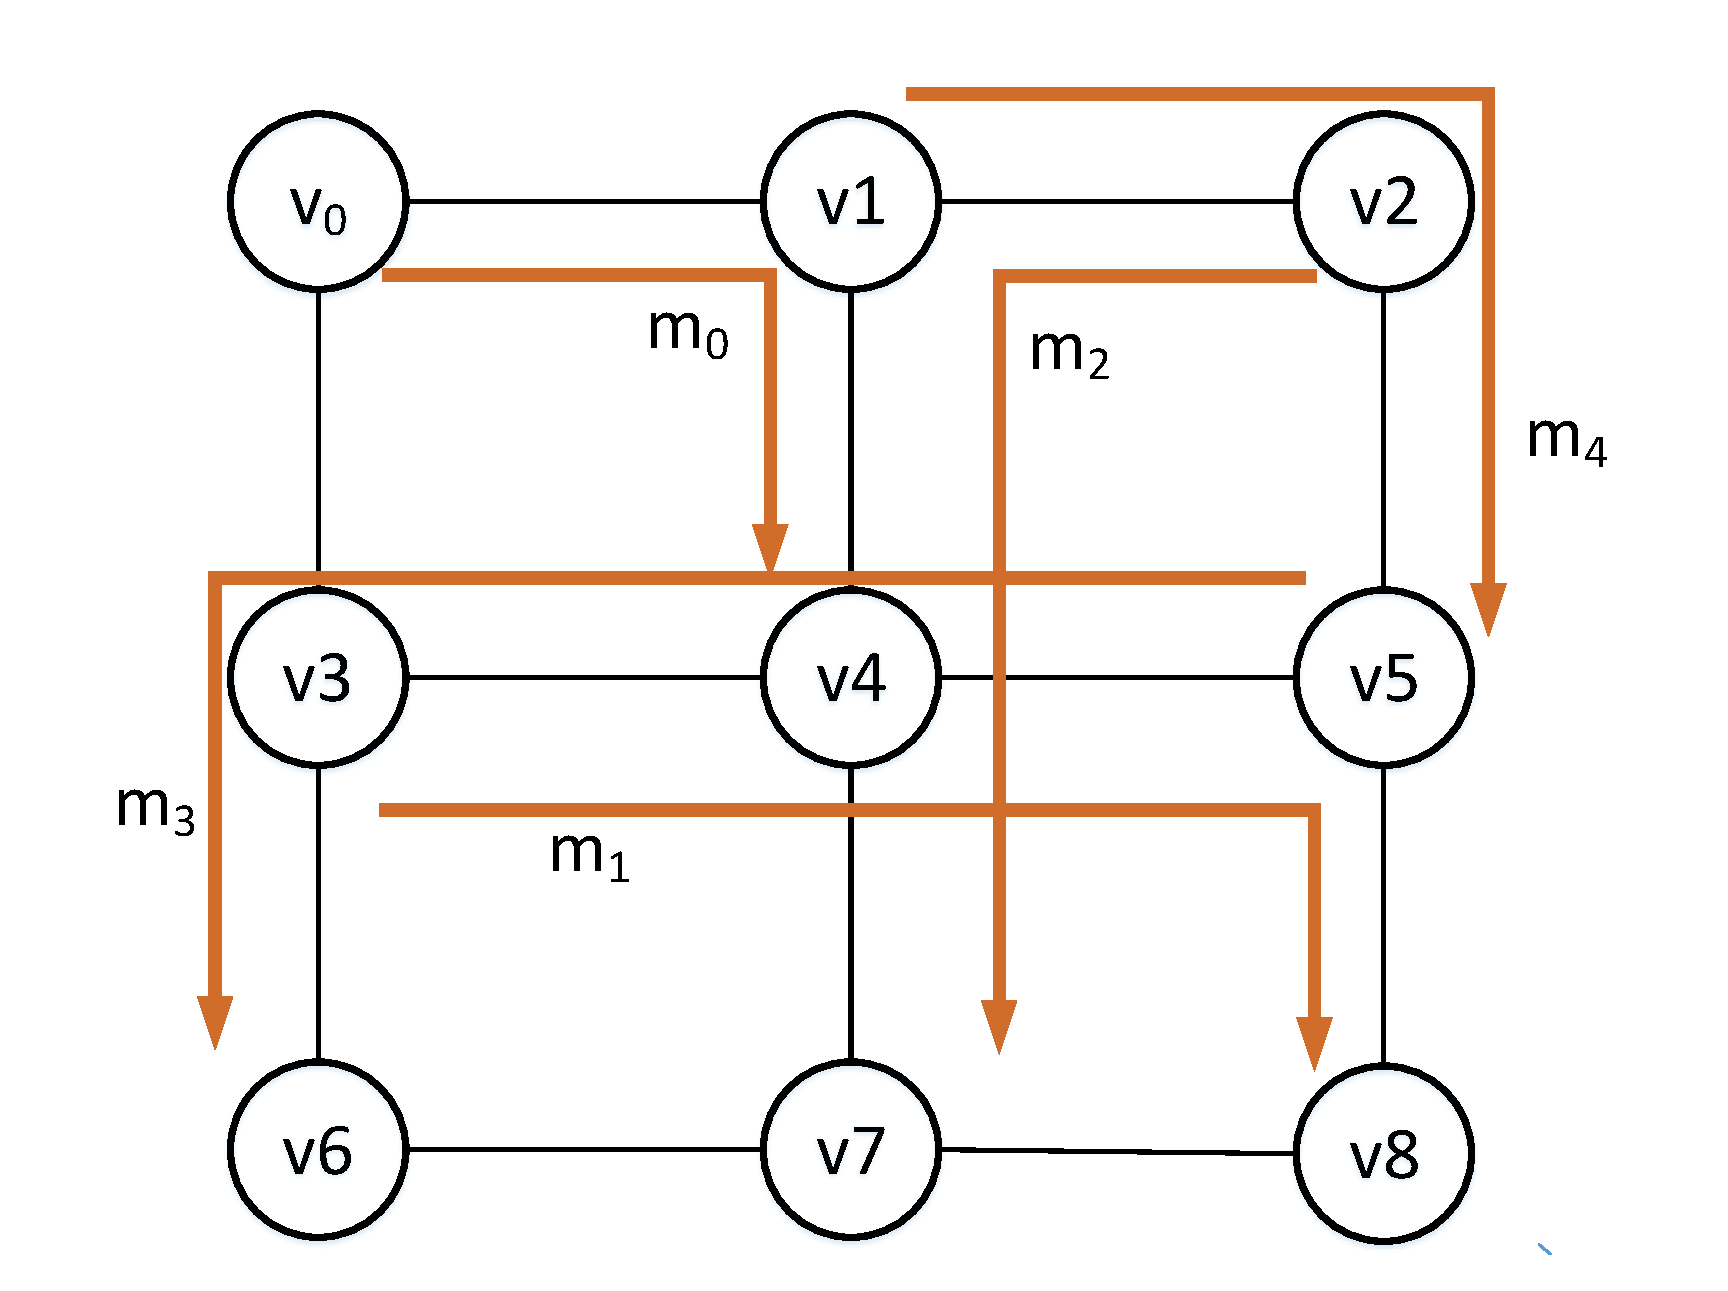
\includegraphics[width=2.5in]{picture/scheduling_example.pdf}
	\caption{An example of communication on the TTNoC}
	\label{f:comm_on_TTNoC}
	
\end{figure}
\begin{table}[!t]
	\renewcommand{\arraystretch}{1.3}
		\newcommand{\tabincell}[2]{\begin{tabular}{@{}#1@{}}#2\end{tabular}}
	%if using array.sty, it might be a good idea to tweak the value of
	% \extrarowheight as needed to properly center the text within the cells
	\caption{An example of scheduling of messages on the TTNoC}
	\label{t:comm_info}
	\centering
	% Some packages, such as MDW tools, offer better commands for making tables
	% than the plain LaTeX2e tabular which is used here.
	\begin{tabular}{|c|c|c|c|c|}
		\hline
			\tabincell{c}{\textbf{Scheduling}\\\textbf{$s_i\in\calS$}}& 
			\tabincell{c}{\textbf{Route}\\ \textbf{$s_i.R$}}& 
			\tabincell{c}{\textbf{Period}\\ \textbf{$s_i.T$}}  & 
			\tabincell{c}{\textbf{Delay }\\ \textbf{$s_i.L$} } & 
			\tabincell{c}{\textbf{Possible Offset}\\ \textbf{$s_i.P_\phi$}} \\
		\hline
		$s_{0}$ & $ \route{r_0}{0}{4}$ & 2 & 1 & $\{0,1\}$\\
		\hline
		$s_{1}$ & $ \route{r_1}{3}{8}$ & 4 & 1 & $\{0,1,2,3\}$\\
		\hline
		$s_{2}$ & $ \route{r_2}{2}{7}$ & 4 & 1 & $\{0,1,2,3\}$\\
		\hline		
		$s_{3}$ & $ \route{r_3}{5}{6}$ & 8 & 2 & $\{0,1,2,3,4,5,6\}$\\
		\hline
		$s_{4}$ & $ \route{r_4}{1}{5}$ & 8 & 1 & $\{0,1,2,3,4,5,6,7\}$\\
		\hline		
	\end{tabular}
\end{table}
\subsection{Genetic Representation}

The genetic algorithm employed in global search, which consists of concepts about gene, chromosome,
 individual and population. 
A population consists of a set of individuals. 
Each individual contains a chromosome and its score respectively.
A chromosome represents a solution to the given question and composes of several genes.
And a gene the unit of chromosome.

In our memetic algorithm,
we adopt the hyperperiod  $Hp(\calS) = LCM\{\calS.\calT\}$
 as the definition of chromosome.
The value of hyperperiod is the least common multiple of the offset among scheduling for messages. 
E.g. the hyperperiod is 8 for the scheduling set on TABLE~\ref{t:comm_info}. 
And a macrotick is defined as the unit of hyperperiod which represents gene.


The location of a gene on a chromosome denotes the offset $ s_i.\phi $ of a message $\tau_i\in\Gamma$.
The $s_i.\phi$ is distributed on a gene.
Hence each chromosome represents a possible allocation for the offset of messages $\calS.\Phi$.
It should be noted that a single gene may consists multiple offset of messages,
 since several messages without contention can be transmitted at same time on the network-based TTNoC.

A set of individuals with respective chromosome composes a population.
The size of population equals the number of individual in the population.
An example of population with two individuals based on TABLE~\ref{t:comm_info} is shown in TABLE~\ref{t:pop}.
The chromosome and gene of individuals are also depicted.
%\begin{figure}[!t]
%	\centering
%	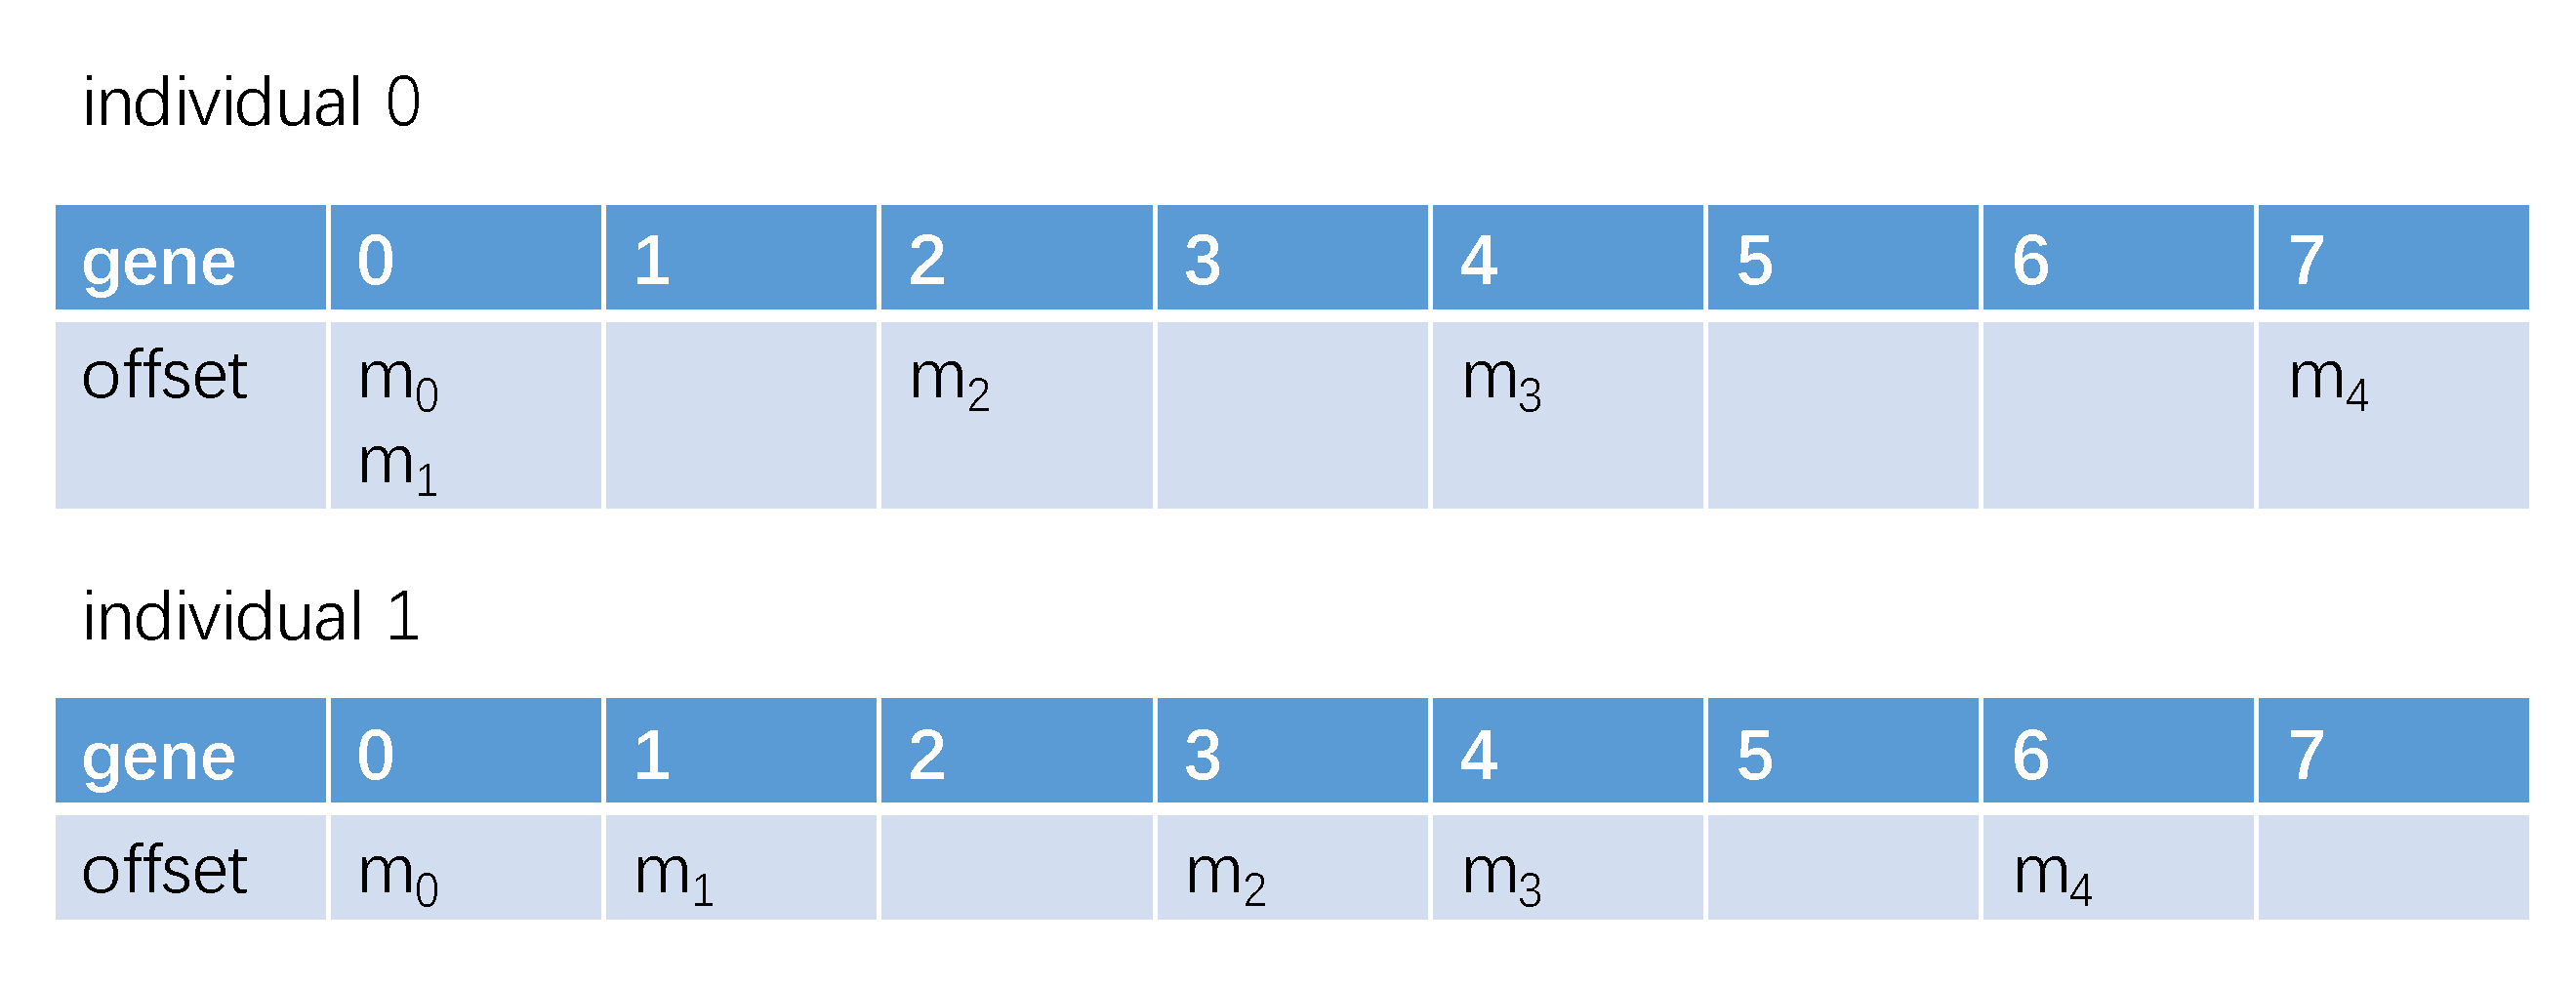
\includegraphics[width=3 in]{picture/2individual}
%	\caption{An example of population with 2 individual}
%	\label{t:pop}
%\end{figure}
\begin{table}[!t]
	\renewcommand{\arraystretch}{1.3}
		\newcommand{\tabincell}[2]{\begin{tabular}{@{}#1@{}}#2\end{tabular}}
	%if using array.sty, it might be a good idea to tweak the value of
	% \extrarowheight as needed to properly center the text within the cells
	\caption{An example of the population consists of 2 individuals}
	\label{t:pop}
	\centering
	% Some packages, such as MDW tools, offer better commands for making tables
	% than the plain LaTeX2e tabular which is used here.
	\begin{tabular}{|c|c|c|c|c|c|c|c|c|}
	\hline
		\textbf{Individual}& 
		\textbf{0} & 
		\textbf{1} & 
		\textbf{2} & 
		\textbf{3} &
		\textbf{4} & 
		\textbf{5} & 
		\textbf{6} & 
		\textbf{7} \\		
	\hline
		$in_0$	&
		\tabincell{c}{ $s_0.\phi$\\$s_1.\phi$}& 
		&
		$s_2.\phi$&
		&
		$s_3.\phi$& 
		& 
		&$s_4.\phi$\\		
	\hline		
		$in_1$	&$s_0.\phi$&$s_1.\phi$&	&$s_2.\phi$&$s_3.\phi$& &$s_4.\phi$&	\\		
	\hline
	\end{tabular}
\end{table}
\subsection{Algorithm Description}

According to the genetic representation, we formal give the algorithm process. The pseudocode is given as follow.

The population $pop$ is synthesized with initialization by $initPop(scale)$.
The size of population $scale$ as well as the maximum iterations $N$ is predefined.
For a scheduling $s_{i}\in\calS$ in the chromosome of a individual,
 the offset $s_i.\phi$ is located randomly among the possible offset $s_i.P_\phi$.
Hence the initial population satisfies the constraints~\ref{c:offset}.
The algorithm is iterative executed until deriving a feasible scheduling or reaching the iteration $N$.

Each individual $in_i$ in $pop$ is marked by the fitness function $fit(in)$. 
The score evaluating chromosome is assigned to its individual.
The less the number of score, the better the chromosome.
Hence the individual with score equals zero represents a feasible scheduling is synthesized.
The detail of fitness function is discussed in Section~\ref{s:fit}.
After evaluating $pop$, the best individual $best$ among the population is selected by $selectBest(pop)$.

Next, the operation of genetic algorithm,
 i.e. $crossover(pop)$ and $mutate(pop)$,
  is deployed as global search.
Then the local search $localSearch(pop)$ is employed if there is no feasible scheduling (individual with score 0) in the $pop$.
The detail of global as well as local search, is discussed in Sections~\ref{s:glo} and~\ref{s:loc}, respectively.

After the global and local search,
 each individual in the $pop$ is evaluated by fitness function again.
And individual with least score in $pop$ is selected as the best one after search $best'$ by $selectBest(pop)$.
The $best$ is compared with $best'$ and select the individual with less score as the new $best$.
 $best'$ compares with previous optimal individual $best$ to derive the individual with less score.
The new population for the next iteration is generated by selection $select(pop,scale)$ according to the score of each individual.
The individual with less score owns more possibility to reserve for the next iteration.
The $select(pop,scale)$ ensures the size of population equals the value of $scale$ in each iteration.

%% \begin{algorithm}[tb]
%% 	\caption{Memetic Algorithm}
%% 	\renewcommand{\algorithmicrequire}{\textbf{Input:}}
%% 	\renewcommand{\algorithmicensure}{\textbf{Output:}}
%% 	\begin{algorithmic}[1]
%% 		\REQUIRE~~\\
%% 		the size of population $scale$\\
%% 		maximum iterations $maxIteration$\\
%% 		\ENSURE~~\\
%% 		Best scheduling $\calS$\\
%% 		\FOR {$i = 0$ to $maxIteration-1$}
%% 			\IF{$i=0$}
%% 			\STATE /*mark the initial population*/
%% 				\STATE generate the	initial population $initialPop$\\
%% 				\STATE mark$(initialPop)$
%% 				\STATE $\mathcal{S}$ = individual with least score \textbf{in} $initialPop$
%% 				\STATE $Pop = initialPop$
%% 			\ELSE
%% 			\STATE /*global search*/
%% 				\STATE crossover($Pop$)
%% 				\STATE mutation($Pop$)
%% 				\STATE mark$(Pop)$
%% 			\ENDIF
%% 			\STATE /*choose the individual best so far after global search*/
%% 			\FORALL {individual $indi$ \textbf{in} $Pop$}		
%% 				\IF{$indi.score<\mathcal{S}.score$}
%% 					\STATE $\mathcal{S}=indi$
%% 				\ENDIF
%% 				\IF{$\mathcal{S}.score==0$}
%% 					\STATE break
%% 				\ENDIF
%% 			\ENDFOR	
%% 			\STATE localSearch($Pop$)
%% 			\STATE mark$(Pop)$
%% 			\STATE /*choose the individual best so far after local search*/
%% 			\FORALL {individual $indi$ \textbf{in} $Pop$}		
%% 				\IF{$indi.score<\mathcal{S}.score$}
%% 					\STATE $\mathcal{S}=indi$
%% 				\ENDIF
%% 				\IF{$\mathcal{S}.score==0$}
%% 					\STATE break
%% 				\ENDIF
%% 			\ENDFOR			
%% 			\STATE select($Pop$, $scale$)
%% 		\ENDFOR
%% 		\RETURN {$\mathcal{S}$}
%% 	\end{algorithmic}
%% \end{algorithm}

\begin{algorithm}[tb]
\caption{Memetic Algorithm}
\renewcommand{\algorithmicrequire}{\textbf{Input:}}
\renewcommand{\algorithmicensure}{\textbf{Output:}}
\begin{algorithmic}[1]
  \REQUIRE~~\\
  the size of population $scale$\\
  maximum number for iterations $N$
  \ENSURE~~\\
  best scheduling offsets $\calS.\Phi$
  
  \STATE $pop \gets initPop(scale)$
  \STATE $best \gets selectBest(pop)$
  \IF{$best.score = 0$}
    \RETURN $\calS.\Phi \gets best.chromosome$
  \ENDIF
  \FOR {$i = 0$ \TO $N-1$}
    \STATE $pop \gets crossover(pop)$
    \STATE $pop \gets mutate(pop)$
    \STATE $pop \gets localSearch(pop)$
    \STATE $best' \gets selectBest(pop)$
    \IF{$best'.score < best.score$}
      \STATE $best \gets best'$
    \ENDIF    
    \IF{$best.score = 0$}
      \STATE break
    \ENDIF

    \STATE $pop \gets select(pop, scale)$
  \ENDFOR

  \RETURN $\calS.\Phi \gets best.chromosome$
\end{algorithmic}
\end{algorithm}	

\subsection{Fitness function \label{s:fit}}

The fitness function is employed to evaluate individuals in the population.
To adopt the fitness function, 
the scenario of overlap among messages should be determined.
And we transform chromosome to represent the duration of messages in a hyperperiod.
Then the score of each individual can be acquired by the fitness function to evaluate the chromosome in Constraint~\ref{c:link}.

According to the predefined routing strategy,
e.g. XY routing~\cite{DBLP:books/daglib/0087651},
the route $s_i.R$ of each scheduling $s_i\in \calS$ for message $\tau_i\in\Gamma$ is derived.
Thus we have the forwarding path per of each message.
By checking the forward routing for each message by Formula~\ref{e:overlap},
the set of scheduling which is overlapped with $s_i$ is derived.
We denote the set of overlapped scheduling $O(s_i)$ for $s_i$ based on Formula~\ref{e:overlap},
and we have that
\begin{equation}
O(s_i) = \{ s_j \mid overlap(s_i,s_j),s_i,s_j\in \calS  \}
\end{equation}
Table~\ref{t:overlap} shows the routing per hop based on XY routing and overlapped set for the scheduling depicted in TABLE~\ref{t:comm_info}.
E.g. since $overlap(s_{0},s_{1}),overlap(s_{0},s_{3})$ are false while $overlap(s_{0},s_{2}),overlap(s_{0},s_{4})$ are true, the overlapped set $O(s_{0})$ is $\{ s_{2},s_{4} \}$. 

\begin{table}[!t]
	\renewcommand{\arraystretch}{1.3}
	\newcommand{\tabincell}[2]{\begin{tabular}{@{}#1@{}}#2\end{tabular}}
	%if using array.sty, it might be a good idea to tweak the value of
	% \extrarowheight as needed to properly center the text within the cells
	\caption{An example of the routing and overlapped set}
	\label{t:overlap}
	\centering
	% Some packages, such as MDW tools, offer better commands for making TABLEs
	% than the plain LaTeX2e tabular which is used here.
	\begin{tabular}{|c||c||c|}
		\hline
		\tabincell{c}{\textbf{Scheduling}\\$s_i\in\calS$} & \tabincell{c}{\textbf{Routing Per Hop}\\$s_i.R$}& \tabincell{c}{\textbf{Overlapped Set}\\ $O(s_i)$}\\
		\hline
		$s_{0}$ & $ \langle 0,1\rangle\langle 1,4\rangle$ 		& $s_{2},s_{4}$ \\
		\hline
		$s_{1}$ & $ \langle 3,4\rangle\langle 4,5\rangle\langle 5,8\rangle$	& $s_{4}$ \\
		\hline
		$s_{2}$ & $ \langle 2,1\rangle\langle 1,4\rangle\langle 4,7\rangle$ 	& $s_{0},s_{4}$ \\
		\hline		
		$s_{3}$ & $ \langle 5,4\rangle\langle 4,3\rangle\langle 3,6\rangle$ 	&$\emptyset$  \\
		\hline
		$s_{4}$ & $ \langle 1,4\rangle\langle 4,5\rangle$ 		& $s_{0},s_{1},s_{2}$ \\
		\hline		
	\end{tabular}
\end{table}

The delay of scheduling $s_i$ in $k$th period $s_i(k)$, is defined by Formula~\ref{e:duration}.
And we have that
\begin{equation}
	D^{Hp}(s_i) = \{ s_i(k) \mid k \in [ 0, Hp(\calS)/s_i.T - 1 ] \}
%s_{i}.\mathcal{H} = \{ {s_{i}^{(v_{a},v_{b})}}(k) \mid k \in [0, \mathcal{M.H} / s_{i}.\mathcal{T} - 1] \}
\end{equation}
where $D^{Hp}(s_i)$ denotes the duration of a scheduling in a hyperperiod.
We define 
 $ D^{Hp}(\calS) = \{ D^{Hp}(s_i) \mid s_i \in \calS \}$
%$\mathcal{M.H}=\{ s_{i}.\mathcal{H} \mid s_{i}\in \mathcal{M} \}$,
 denotes the set of duration for messages in a hyperperiod. 
Therefore the complete duration in a hyperperiod for all the scheduling of message is determined.
TABLE~\ref{t:duration} is an example of the complete duration in a hyperperiod,
 based on two individuals in TABLE~\ref{t:pop}.
The scheduling model of messages is shown in TABLE~\ref{t:comm_info}.

%\begin{figure}[!t]
%	\centering
%	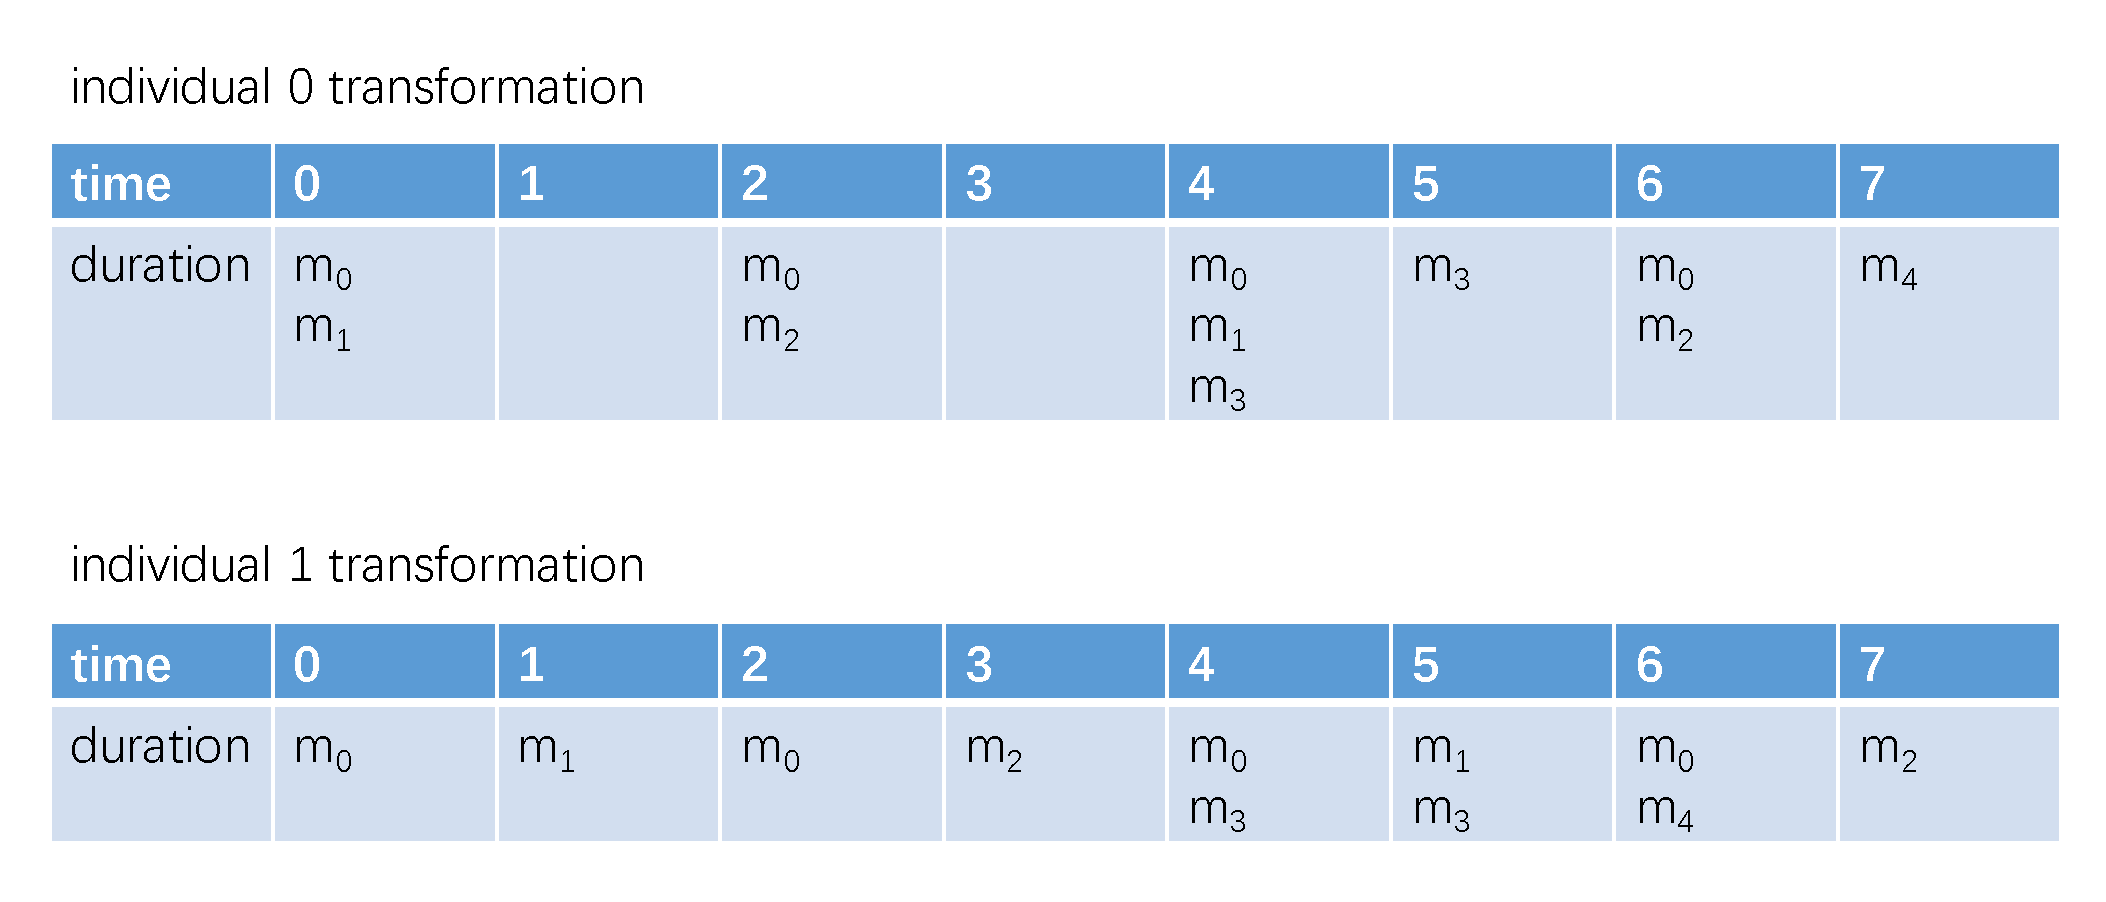
\includegraphics[width=3in]{picture/individual_transformation.pdf}
%	\caption{The duration of the messages in the hyperperiod}
%	\label{f:duration}
%\end{figure}
\begin{table}[!t]
	\renewcommand{\arraystretch}{1.3}
	\newcommand{\tabincell}[2]{\begin{tabular}{@{}#1@{}}#2\end{tabular}}
	%if using array.sty, it might be a good idea to tweak the value of
	% \extrarowheight as needed to properly center the text within the cells
	\caption{An example of transform of chromosome to represent duration of scheduling}
	\label{t:duration}
	\centering
	% Some packages, such as MDW tools, offer better commands for making tables
	% than the plain LaTeX2e tabular which is used here.
	\begin{tabular}{|c|c|c|c|c|c|c|c|c|}
		\hline
		\textbf{Individual}& 
		\textbf{0} & 
		\textbf{1} & 
		\textbf{2} & 
		\textbf{3} &
		\textbf{4} & 
		\textbf{5} & 
		\textbf{6} & 
		\textbf{7} \\		
		\hline
		$in_0$&
		\tabincell{c}{$\tau_0$\\$\tau_1$}&
		&
		\tabincell{c}{$\tau_0$\\$\tau_2$}&
		&
		\tabincell{c}{$\tau_0$\\$\tau_1$\\$\tau_3$}&
		$\tau_3$&
		\tabincell{c}{$\tau_0$\\$\tau_2$}&
		$\tau_4$\\		
		\hline	
		$in_1$&
		$\tau_0$&
		$\tau_1$&
		$\tau_0$&
		$\tau_2$&
		\tabincell{c}{$\tau_0$\\$\tau_3$}&
		\tabincell{c}{$\tau_1$\\$\tau_3$}&
		\tabincell{c}{$\tau_0$\\$\tau_4$}&
		$\tau_2$\\
		\hline
	\end{tabular}
\end{table}

For $s_{i},s_{j}\in \calS, s_{i}\neq s_{j}$,
if $s_i$ and $s_j$ are overlapped,
the conflict times between them should be derived to evaluate the chromosome.
For each $s_{i}\in \calS$,
 we define $C(s_{i})$ to derive the set of scheduling conflicted with $s_{i}$. 
So we have that
\begin{equation}
	C(s_i) = \{ s_j \mid D^{Hp}(s_i) \cap D^{Hp}(s_j) \neq \emptyset  ,s_j\in O(s_i) \}
%C(s_{i}) = \{(s_{i},s_{j})\rightarrow n_{ij}\mid m_j\in O(s_{i}),s_{i},s_{j}\in \mathcal{M}\}
\end{equation}
If there is no conflict scheduling with $s_i$ on the its duration,
$C(s_i)\in \emptyset$.   
A function to count the conflict times between $s_i$ and $s_j$ is defined as
\begin{equation}
	conflict(s_i,s_j) = |D^{Hp}(s_i) \cap D^{Hp}(s_j)|
\end{equation}
%We define the mapping $(s_{i},s_{j})\rightarrow n_{ij}$, where $(s_{i},s_{j})$ is the conflict communication and $n_{ij}$ is the number of gene which $s_{i}$ coexist with $s_{j}$ on a chromosome is $n_{ij}$, which denotes the conflict times between $s_{i}$ and $s_{j}$.

We define the total conflict times for $s_{i}$ as $times(s_i)$. And we have that
\begin{equation}
	times(s_i)=\sum_{ s_j \in C(s_i) } conflict(s_i,s_j)
\end{equation}

We define $C(\calS) = \{ s_i \mid C(s_i) \notin \emptyset \} $ to denote the set of conflictive scheduling in a chromosome.

According to $C(\calS)$ the conflict times among any two of scheduling for messages   on the chromosome is determined.
The fitness function assigns a score to each individual.
The output of fitness function is total number of conflicts in $C(\calS)$.
Thus for a individual $in$, we have that
\begin{equation}
	fit(in)=\sum_{s_i \in C(\calS)} {times(s_i)}
\end{equation}

Since the score represents the conflict times, the less the score the better the individual.
E.g. the score of two individual in Fig.~\ref{t:pop} is shown in TABLE~\ref{t:fitness}. 

\begin{table}[!t]
	\renewcommand{\arraystretch}{1.3}
	\newcommand{\tabincell}[2]{\begin{tabular}{@{}#1@{}}#2\end{tabular}}
	%if using array.sty, it might be a good idea to tweak the value of
	% \extrarowheight as needed to properly center the text within the cells
	\caption{An example of marking two individuals by the fitness function}
	\label{t:fitness}
	\centering
	% Some packages, such as MDW tools, offer better commands for making TABLEs
	% than the plain LaTeX2e tabular which is used here.
	\begin{tabular}{|c||c||c||c|}
		\hline
		\tabincell{c}{\textbf{Individual}\\$in$}&\tabincell{c}{\textbf{Conflict}\\$C(s_i)$} &\tabincell{c}{\textbf{Conflict Times}\\$times(s_i)$} &\tabincell{c}{\textbf{Score}\\$fit(in)$}\\
		\hline 
		$in_0$ &$s_0,s_2$ & \tabincell{c}{$times(s_0)=2$\\$times(s_2)=2$} &4\\
		\hline
		$in_1$ & $s_0,s_4$& \tabincell{c}{$times(s_0)=1$\\$times(s_4)=1$} &2\\
		\hline
		\end{tabular}	
\end{table}

\subsection{Global search strategy \label{s:glo}}

The general operation in genetic algorithm such as crossover and mutate,
  is used in the step of global search. 

For operation of crossover,
 we employ two of the individuals $in_i$ and $in_j$ among the population as parents to join the crossover in terms of their score.
The lower score of the individual,
 the higher possibility for this individual to be selected as parent.
The crossover generates a new individual called child, and its chromosome depends on the parents.
The individual of parents with lower score owns the higher possibility to determine the offset location $s_i.\phi$ for $s_i\in\calS$ on the chromosome of child.
For parents $in_i$ and $in_j$, we have the function
\begin{equation}
	possibility(in_i)=1-\frac{in_i}{in_i+in_j}
\end{equation}
to represent the possibility for $in_i$ as a parent to determine the offset in the chromosome of child.
Table~\ref{t:crossover} shows an process of crossover.
The $in_2$ is generated by crossover based on the two individuals in Fig.~\ref{t:pop} as parents.
Because the score of $in_0$ is 4 while $in_1$ is 2,
 $in_0$ owns 67\% while $in_0 $ have 33\% of possibility to decide the offset when locating each scheduling $s_i\in\calS$.
The chromosome of $in_2$ consists of the offset of $s_0,s_2,s_3$ from $in_1$ and $s_1,s_4$ from $in_0$.
%\begin{figure}[!t]
%	\centering
%	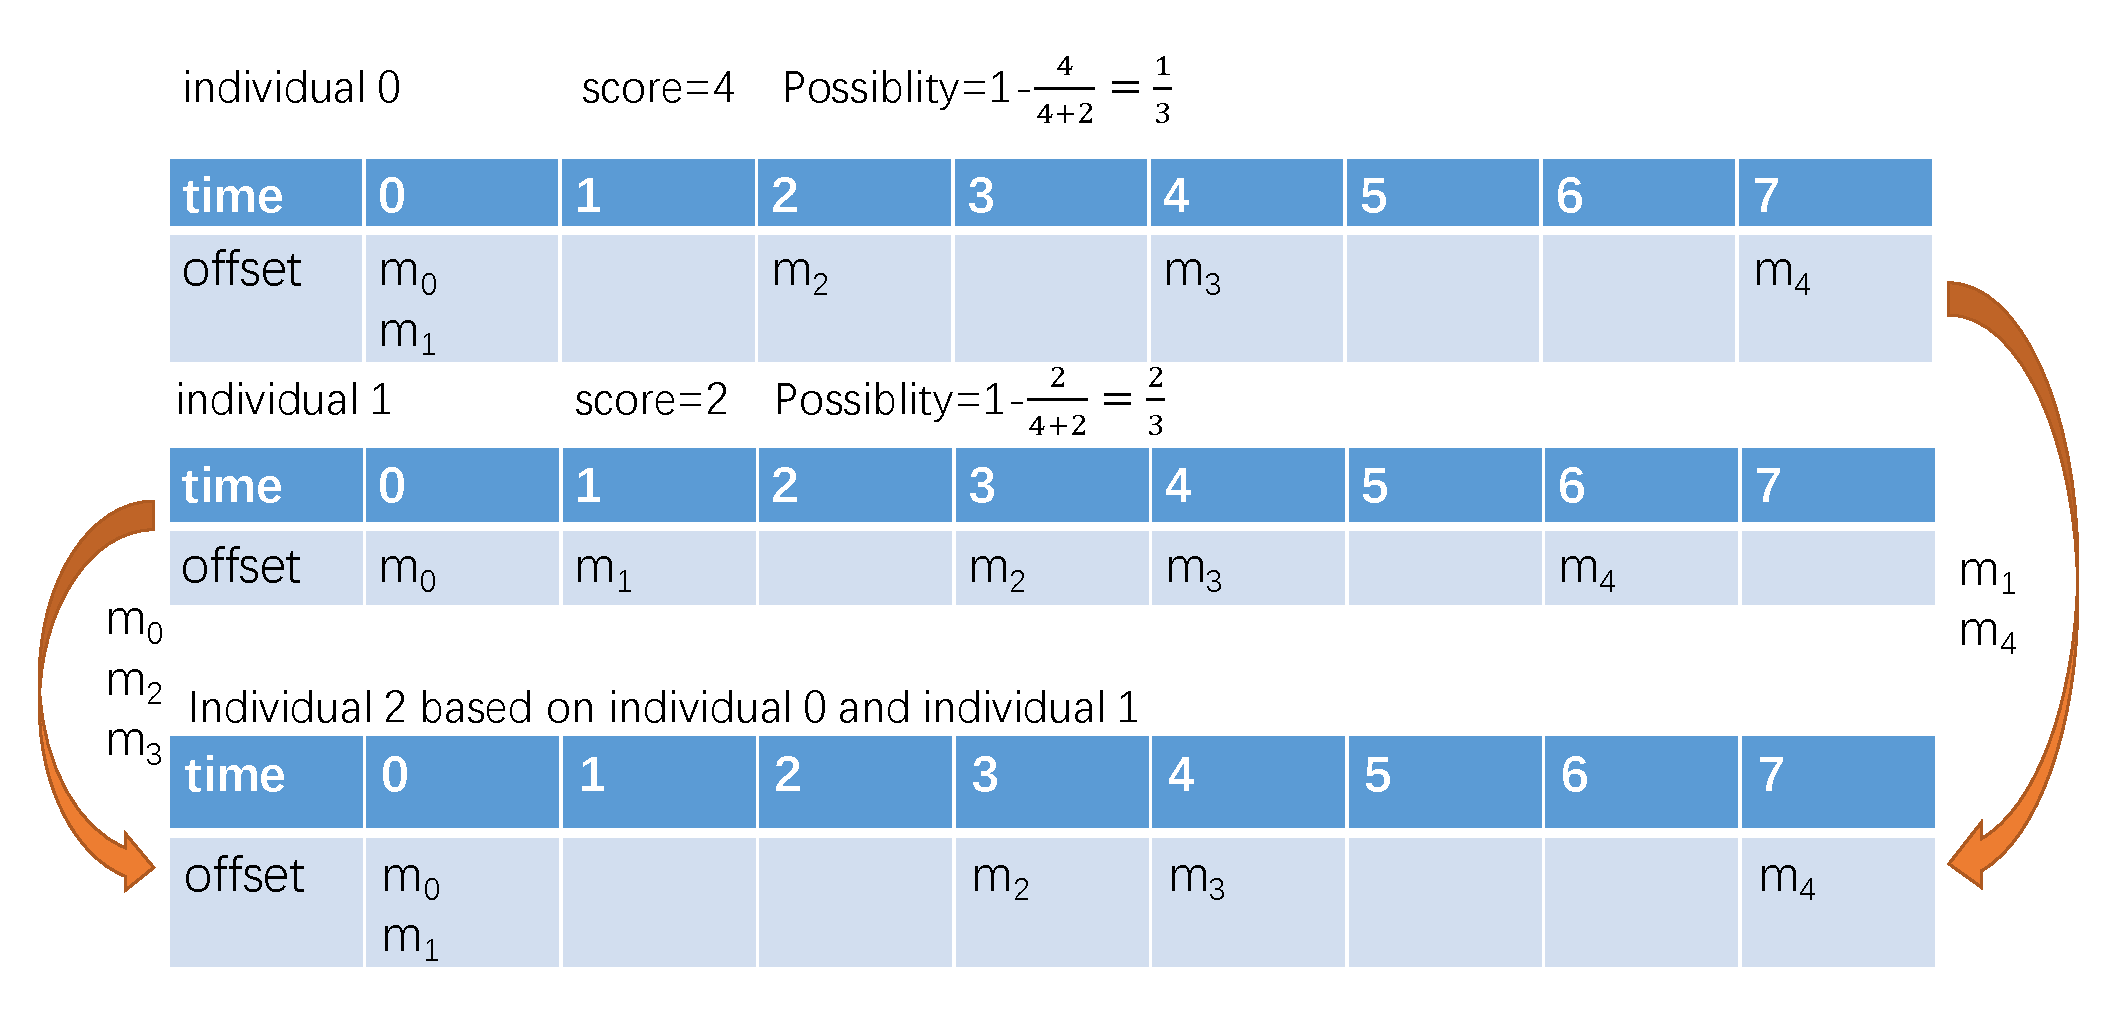
\includegraphics[width=3in]{picture/crossover.pdf}
%	\caption{An example of crossover employed individuals in Fig.~\ref{t:pop} as parents}
%	\label{f:crossover}
%\end{figure}
\begin{table}[!t]
	\renewcommand{\arraystretch}{1.3}
	\newcommand{\tabincell}[2]{\begin{tabular}{@{}#1@{}}#2\end{tabular}}
	%if using array.sty, it might be a good idea to tweak the value of
	% \extrarowheight as needed to properly center the text within the cells
	\caption{An example of crossover}
	\label{t:crossover}
	\centering
	% Some packages, such as MDW tools, offer better commands for making tables
	% than the plain LaTeX2e tabular which is used here.
	\begin{tabular}{|c|c|c|c|c|c|c|c|c|}
		\hline
		\textbf{Parent}& 
		\textbf{0} & 
		\textbf{1} & 
		\textbf{2} & 
		\textbf{3} &
		\textbf{4} & 
		\textbf{5} & 
		\textbf{6} & 
		\textbf{7} \\		
		\hline
		$in_0$	&\tabincell{c}{$s_0.\phi$\\$s_1.\phi$}&	&$s_2.\phi$&	&$s_3.\phi$& & &$s_4.\phi$\\		
		\hline		
		$in_1$	&$s_0.\phi$&$s_1.\phi$&	&$s_2.\phi$&$s_3.\phi$& &$s_4.\phi$&	\\		
		\hline
		\hline
			\textbf{Child}& 
			\textbf{0} & 
			\textbf{1} & 
			\textbf{2} & 
			\textbf{3} &
			\textbf{4} & 
			\textbf{5} & 
			\textbf{6} & 
			\textbf{7} \\		
			\hline
			$in_2$	&\tabincell{c}{$s_0.\phi$\\$s_1.\phi$}&	& &$s_2.\phi$&$s_3.\phi$& & &$s_4.\phi$\\			
		\hline
	\end{tabular}
\end{table}

The operation of mutate random selects an offset $s_i.\phi$ of scheduling $s_i\in\calS$.
Then reallocating a new offset randomly in its possible offset $s_i.P_\phi$.
TABLE~\ref{t:mutation} is an example of operation of mutate.
It is noticed that the probability of mutate for each individual in our implement is 50\%.
%\begin{figure}[!t]
%	\centering
%	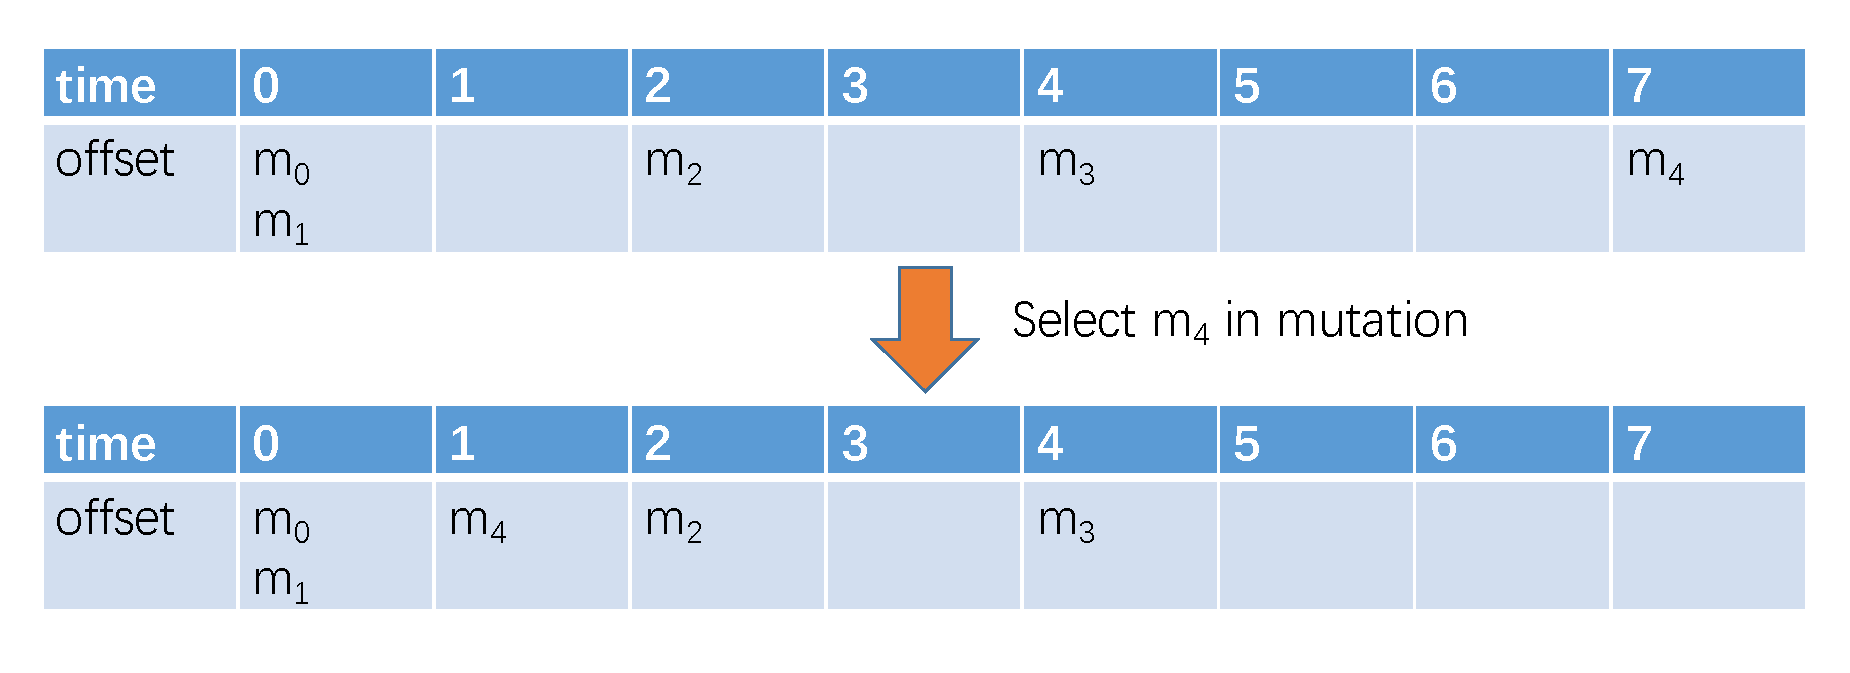
\includegraphics[width=3in]{picture/mutation.pdf}
%	\caption{An example of mutation}
%	\label{f:mutation}
%\end{figure}
\begin{table}[!t]
	\renewcommand{\arraystretch}{1.3}
	\newcommand{\tabincell}[2]{\begin{tabular}{@{}#1@{}}#2\end{tabular}}
	%if using array.sty, it might be a good idea to tweak the value of
	% \extrarowheight as needed to properly center the text within the cells
	\caption{An example of mutate}
	\label{t:mutation}
	\centering
	% Some packages, such as MDW tools, offer better commands for making tables
	% than the plain LaTeX2e tabular which is used here.
	\begin{tabular}{|c|c|c|c|c|c|c|c|c|}
		\hline
		\textbf{Before}& 
		\textbf{0} & 
		\textbf{1} & 
		\textbf{2} & 
		\textbf{3} &
		\textbf{4} & 
		\textbf{5} & 
		\textbf{6} & 
		\textbf{7} \\		
		\hline
		$in_0$	&\tabincell{c}{$s_0.\phi$\\$s_1.\phi$}&	&$s_2.\phi$&	&$s_3.\phi$& & &$s_4.\phi$\\		
		\hline
		\hline
		\textbf{After}& 
		\textbf{0} & 
		\textbf{1} & 
		\textbf{2} & 
		\textbf{3} &
		\textbf{4} & 
		\textbf{5} & 
		\textbf{6} & 
		\textbf{7} \\		
		\hline
		$in_0$	&\tabincell{c}{$s_0.\phi$\\$s_1.\phi$}&$s_4.\phi$&$s_2.\phi$&	&$s_3.\phi$& & &\\			
		\hline
	\end{tabular}
\end{table}


\subsection{Local search strategy \label{s:loc}}

Before the local search for each individual,
 the scheduling $s_i\in\calS$ with the maximum value of $times(s_i)$ is selected as local search element.
If there are two or more individuals with the maximum conflict times,
 the element to be searched is select stochastically among them.
Then the offset $s_i.\phi$ of selected $s_i$ is reallocated in its possible offset $s_i.P_\phi$.
Each reallocated individual is a candidate which can update the previous individual.
After marking all of the candidate, the individual with minimum score replaces the previous individual.

TABLE~\ref{t:local} shows an example of local search for $in_0$ in Fig.~\ref{t:pop}.
According to the $T(\calS)$ of individual 0 in TABLE~\ref{t:fitness},
 we random select $s_0$ as the element. 
Since the possible offset $s_i.P_\phi$ of $s_0.\phi$ is 0 and 1 shown in TABLE~\ref{t:comm_info},
  we locate the the scheduling $s_0$ for message $m_0$ on its possible offset, gene 0 and gene 1 respectively.
After marking two of individual with varying offset $s_0.\phi$,
 we select the individual which score is 2 as the updated $in_0$ because this individual owns minimum score among the candidates which reallocate the $s_0,\phi$.
%\begin{figure}[!t]
%	\centering
%	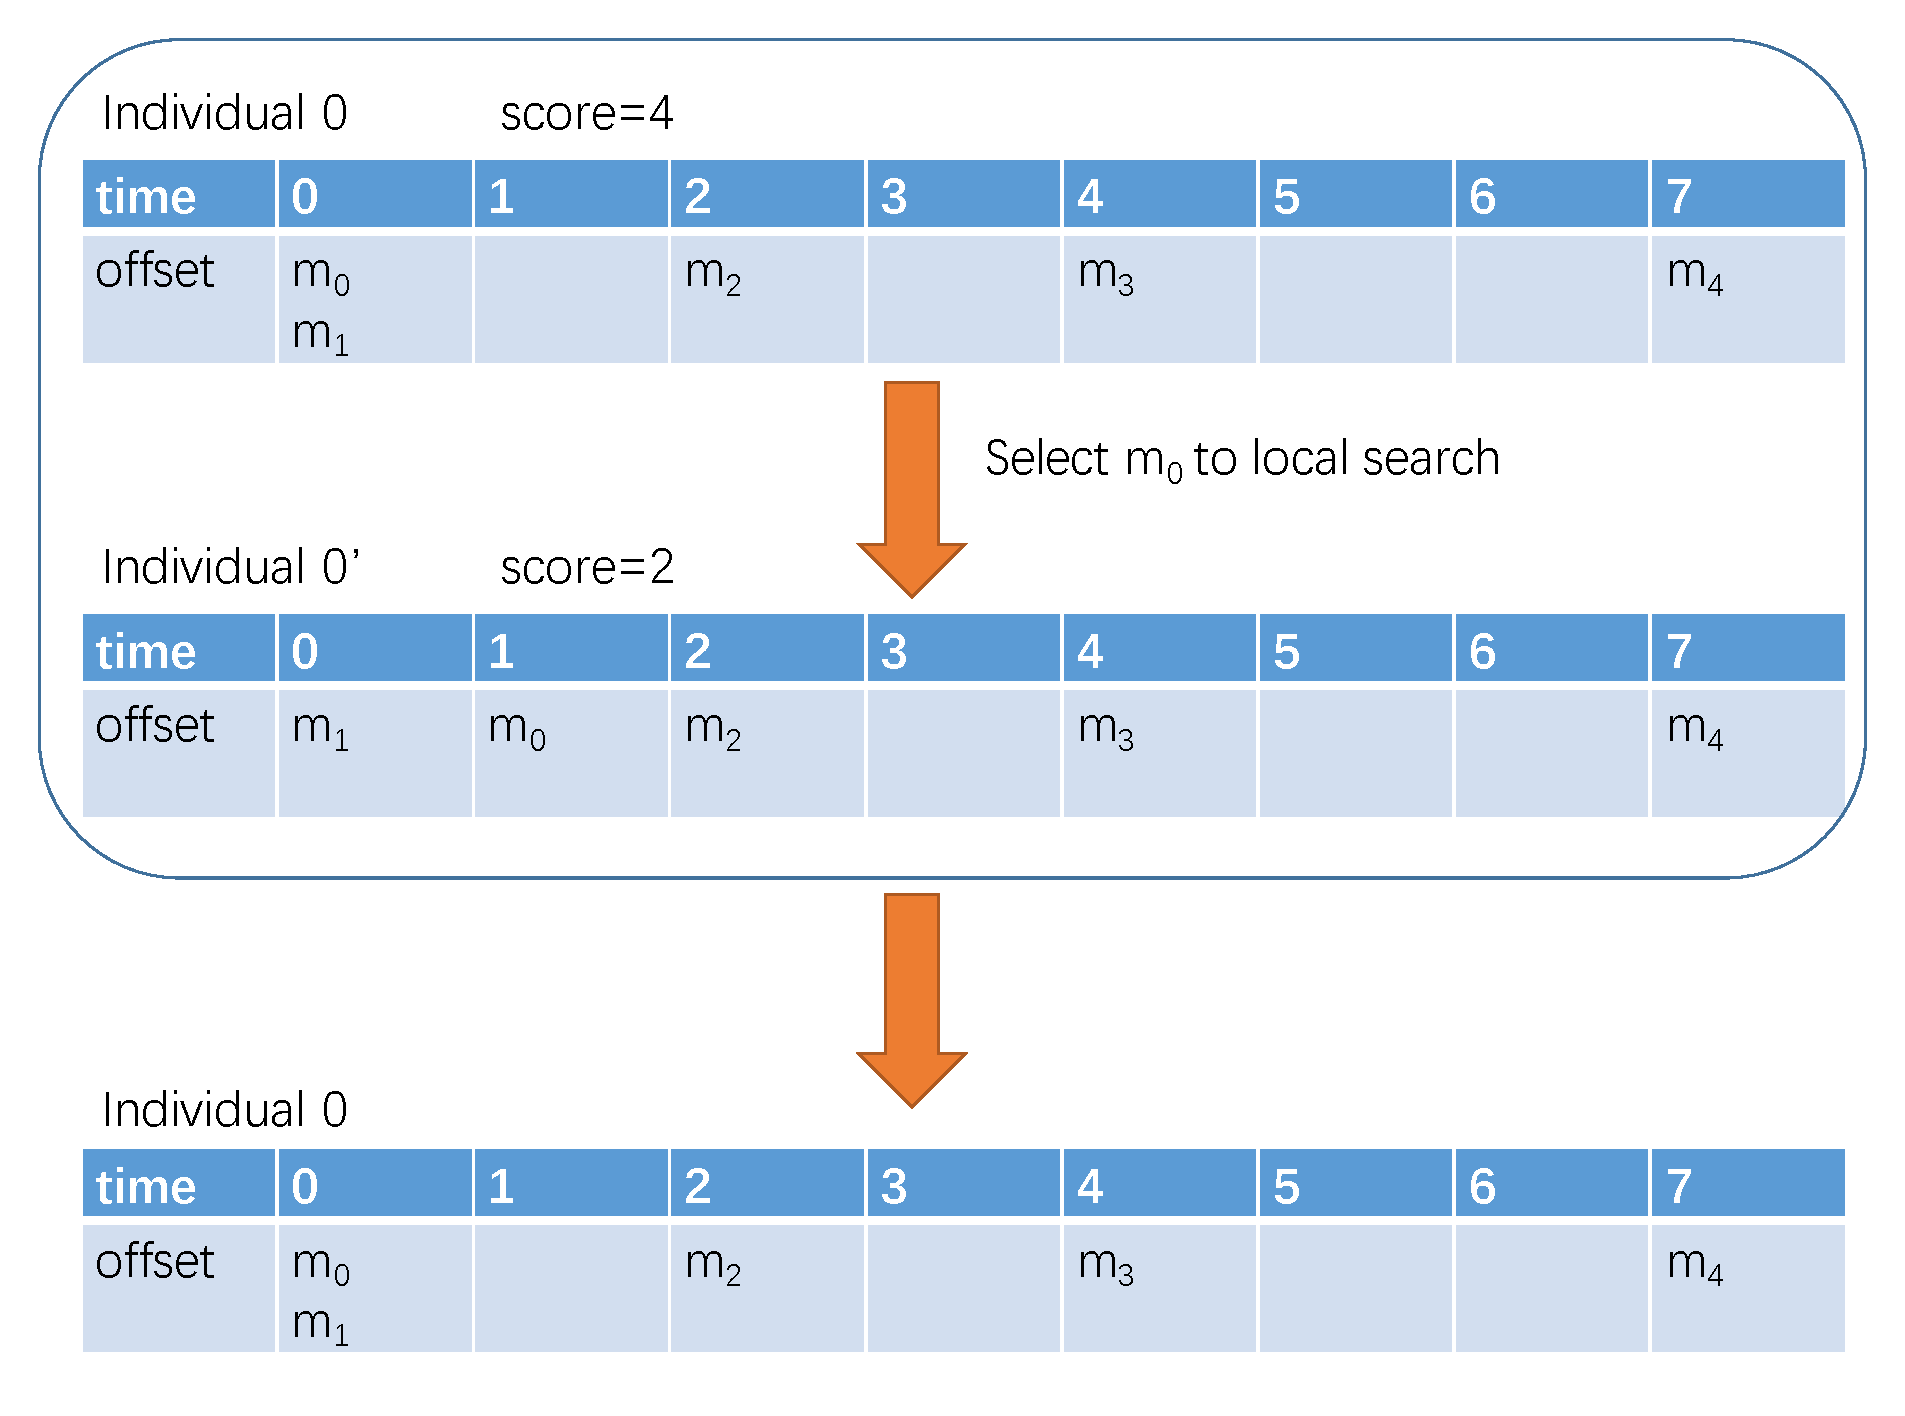
\includegraphics[width=3in]{picture/local.pdf}
%	\caption{An example of local search}
%	\label{f:local}
%\end{figure}
\begin{table}[!t]
	\renewcommand{\arraystretch}{1.3}
	\newcommand{\tabincell}[2]{\begin{tabular}{@{}#1@{}}#2\end{tabular}}
	%if using array.sty, it might be a good idea to tweak the value of
	% \extrarowheight as needed to properly center the text within the cells
	\caption{An example of local search of $s_0$ as element}
	\label{t:local}
	\centering
	% Some packages, such as MDW tools, offer better commands for making tables
	% than the plain LaTeX2e tabular which is used here.
	%\tabincell{c}
	\begin{tabular}{|c||c||c||c||c||c||c||c||c|}
		\hline
		\textbf{Before}& 
		\textbf{0} & 
		\textbf{1} & 
		\textbf{2} & 
		\textbf{3} &
		\textbf{4} & 
		\textbf{5} & 
		\textbf{6} & 
		\textbf{7} \\		
		\hline
		$in_0$	&\tabincell{c}{$s_0.\phi$\\$s_1.\phi$}&	&$s_2.\phi$&	&$s_3.\phi$& & &$s_4.\phi$\\		
		\hline
		\hline
		\textbf{Score}& 
		\textbf{0} & 
		\textbf{1} & 
		\textbf{2} & 
		\textbf{3} &
		\textbf{4} & 
		\textbf{5} & 
		\textbf{6} & 
		\textbf{7} \\		
		\hline
		$4$	&\tabincell{c}{$s_0.\phi$\\$s_1.\phi$}&	&$s_2.\phi$&	&$s_3.\phi$& & &$s_4.\phi$\\
		\hline
		$2$	&$s_1.\phi$&$s_0.\phi$&$s_2.\phi$&	&$s_3.\phi$& & &$s_4.\phi$\\		
		\hline
		\hline		
		\textbf{After}& 
		\textbf{0} & 
		\textbf{1} & 
		\textbf{2} & 
		\textbf{3} &
		\textbf{4} & 
		\textbf{5} & 
		\textbf{6} & 
		\textbf{7} \\		
		\hline
		$in_0$&$s_1.\phi$&$s_0.\phi$&$s_2.\phi$&	&$s_3.\phi$& & &$s_4.\phi$\\		
		\hline
	\end{tabular}
\end{table}

In our implement,
 we naively traverse all the possible offset in $s_i.P_\phi$.
However for improving efficiency,
 many other algorithms in local search can be applied,
  i.e. tabu search, simulated annealing.
And a varying local search strategy may increase the performance of the memetic algorithm.

\section{Evaluations \label{s:evalu}}

\subsection{Experiments Configurations}
%The mapping between a message and a communication node $\{ <\tau_{i} , v_{j}>\mid \tau_{i}\in\Gamma,v_{j}\in\mathcal{V} \}$ is given. Each message $\tau_{i}\in\Gamma$ is allocated to a specific process element(communication node) $v_{i}\in\mathcal{V}$, thus the source node $v_{a}$ and sink node $v_{b}$ in $(v_{a},v_{b})\in \mathcal{L}$ are determined.

%The routing strategy of each message is given. Therefore the link $(v_{a},v_{b})$ and the set of switches for forwarding the message is deterministic.To transmit a message $ \tau_{i}\in\Gamma $, the forwarding path is split in terms of hops by specific routing, i.e. $(v_{a},v_{b})=\{(v_{a},v_{s}),(v_{s},v_{n}),\dots,(v_{p},v_{q}),(v_{q},v_{b})\}$. 

%The switching technique is store-and-forward.

%The latency of forwarding in switch as well as the propagation latency on links is constant.

%In our experiment, for simplicity, the relative deadline is equal to the period for each message. The 2-ary mesh network is used and we randomly generate the mapping on the network. The X-Y routing is adopted as the routing strategy. And the relative deadline for each message equal its period. However the algorithm we introduced can be extended to resolve the scheduling problem with the general topology and arbitrary deterministic routing.


The network architecture we employed for simulation is 2D mesh network which scale is $3\times 3$, $5\times 5$ and $7\times 7$,
 with 9, 25 and 49 switching nodes respectively.
Our algorithm is implemented in JAVA and is running on a Windows with 4GHz CPU and 12GB memory.
We compare the memetic algorithm with the general genetic algorithm without local search. 

The number of scheduling of messages in our evaluation is from 5 to 50.
Each scheduling of message owns its period and delay which is random generated.
We test 15 cases in each scale of architecture with different number of messages.
The size of population we configured is 100.
So there are 100 initial individuals.
And the maximum iterate times we set is 100.
The memetic algorithm will finish when synthesizing a individual with score 0 that represents a feasible scheduling,
 otherwise the algorithm will execute until the iterate times 100.
The case which executes exceeds an hour will be regarded as \emph{overtime}.

\subsection{Failed Scheduling Rate}
We define the failed scheduling of messages $\calS.\Phi_{fail}$ as the minimum number of messages.
The messages which failed to scheduling block the scheduling of other messages.
If the subset of failed scheduling is removed from the given set of scheduling on the TTNoC,
 the remaining messages will be scheduled, which denotes $\calS.\Phi_{sche}$.

We define the rate of failed scheduling as
\begin{equation}
	R_{fail} = \frac{|\calS.\Phi_{fail}|}{|\calS.\Phi|}
\end{equation}

Fig.~\ref{f:fail} shows the $R_{fail}$ for variable type of test cases by MA and GA, denoted as $R_{fail}({MA})$ and $R_{fail}(GA)$  respectively. 
It should be noted that the rate is the average result of the 15 test cases for the same architecture and the number of messages but varying generated messages.

As can be seen,
  the rate of failed scheduled messages by the GA is much more than the MA, especially when the scale of messages is relatively large.
E.g. for the case of 50 messages in $3\times 3$ TTNoC,
 the failed communication percentage is 17.3\% for genetic algorithm while 8\% for memetic algorithm.
It is proposed that the local search in the MA is the key step to significantly improve the performance of GA.

And it is clear that $R_{fail}$ decreases when the scale of TTNoC architecture increasing. 
The reason is that the link resource increases with the growth of architecture,
 resulting of decreasing the possibility of contention among the messages transmission on the TTNoC.
It also presents that the failed communication rate increases when the number of messages on the TTNoC increasing.
It is because that the limited link resources have to transmit more messages when there is more communication on the TTNoC.

To compare the performance of GA and MA,
 we define that
\begin{equation}
	Gain=\frac{R_{fail}(MA)}{R_{fail}(GA)}
\end{equation}
to represent the failed scheduling decreasing comparing MA with GA.
TABLE~\ref{t:performance} depicts the $Gain$ of MA compared with GA.
As we can see, The $R_{fail}(MA)$ is about 30\% of the $R_{fail}(GA)$.

\begin{figure}[!t]
	\centering
	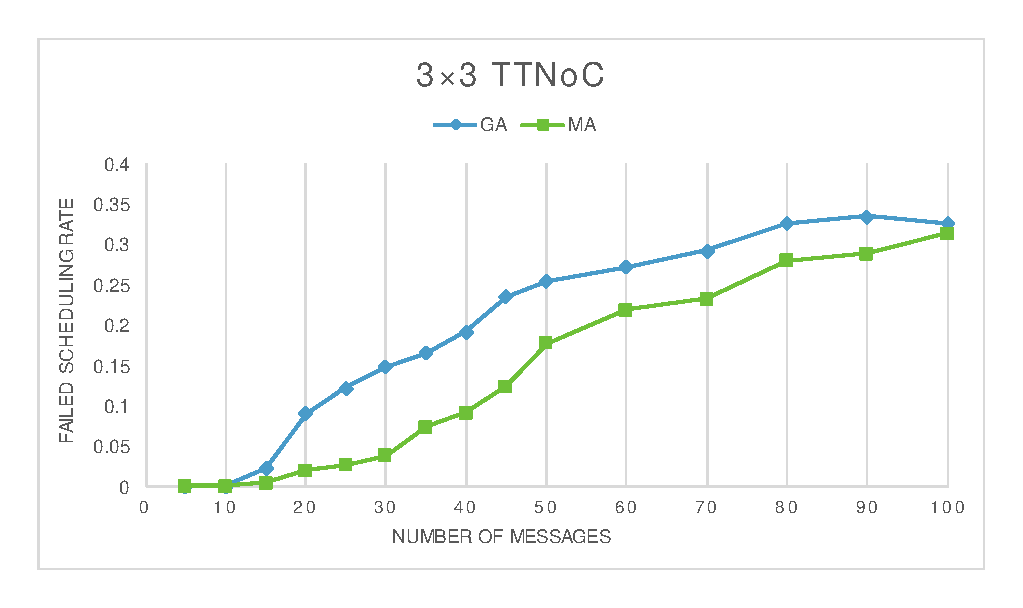
\includegraphics[width=3in]{picture/33TTNOC}
		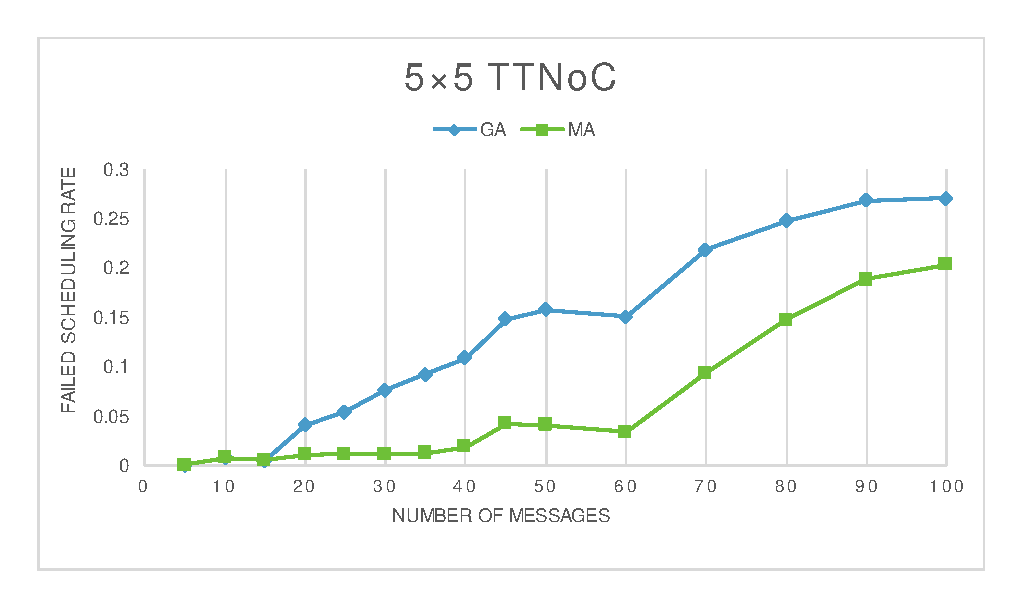
\includegraphics[width=3in]{picture/55TTNOC}
			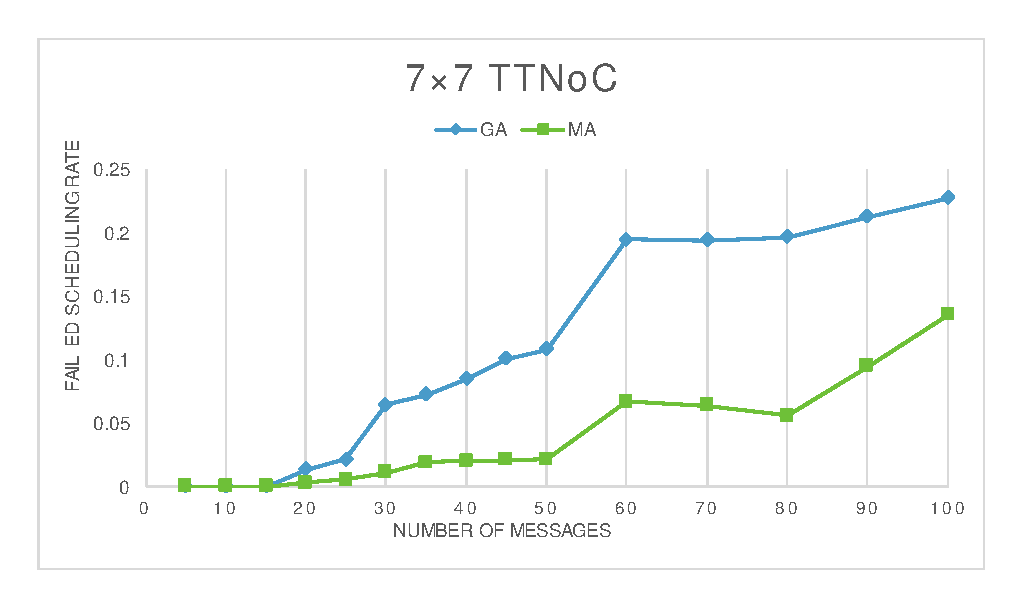
\includegraphics[width=3in]{picture/77TTNOC}
	\caption{The rate of failed scheduling}
	\label{f:fail}
\end{figure}

\subsection{Feasible Cases}
\begin{table}[!t]
	\renewcommand{\arraystretch}{1.3}
	%if using array.sty, it might be a good idea to tweak the value of
	% \extrarowheight as needed to properly center the text within the cells
	\caption{The average rate of failed scheduling in different architecture }
	\label{t:performance}
	\centering
	% Some packages, such as MDW tools, offer better commands for making TABLEs
	% than the plain LaTeX2e tabular which is used here.
	\begin{tabular}{|c||c||c||c|}
		\hline
		\textbf{Architecture} & \textbf{$R_{fail}(MA)$} &\textbf{$R_{fail}(GA)$} & \textbf{Gain}\\
		\hline 
		$3\times 3$ TTNoC&0.0557& 0.1232&	0.4521		
		\\
		\hline
		$5\times 5$ TTNoC& 0.0154	& 0.0685&0.2248\\
		\hline
		$7\times 7$ TTNoC& 0.010& 	0.0465&	0.2165\\
		\hline		
		\hline
		\textbf{Average }& 	0.0271 &0.0794&0.2978\\
		\hline
	\end{tabular}	
\end{table}
We consider the number of feasible case in each experiment type.
The case is feasible if synthesized scheduling $\calS.\Phi$ are scheduled without link contention,
 otherwise we consider the case is infeasible case.
Fig.~\ref{f:feasible} presents the result of number of feasible cases after schedule synthesis.
For simple test cases with less than 15 messages,
 almost cases is feasible.
But for complexed test cases more than 30 messages, it is hard for the algorithms to find a feasible scheduling.
\begin{figure}[!t]
	\centering
	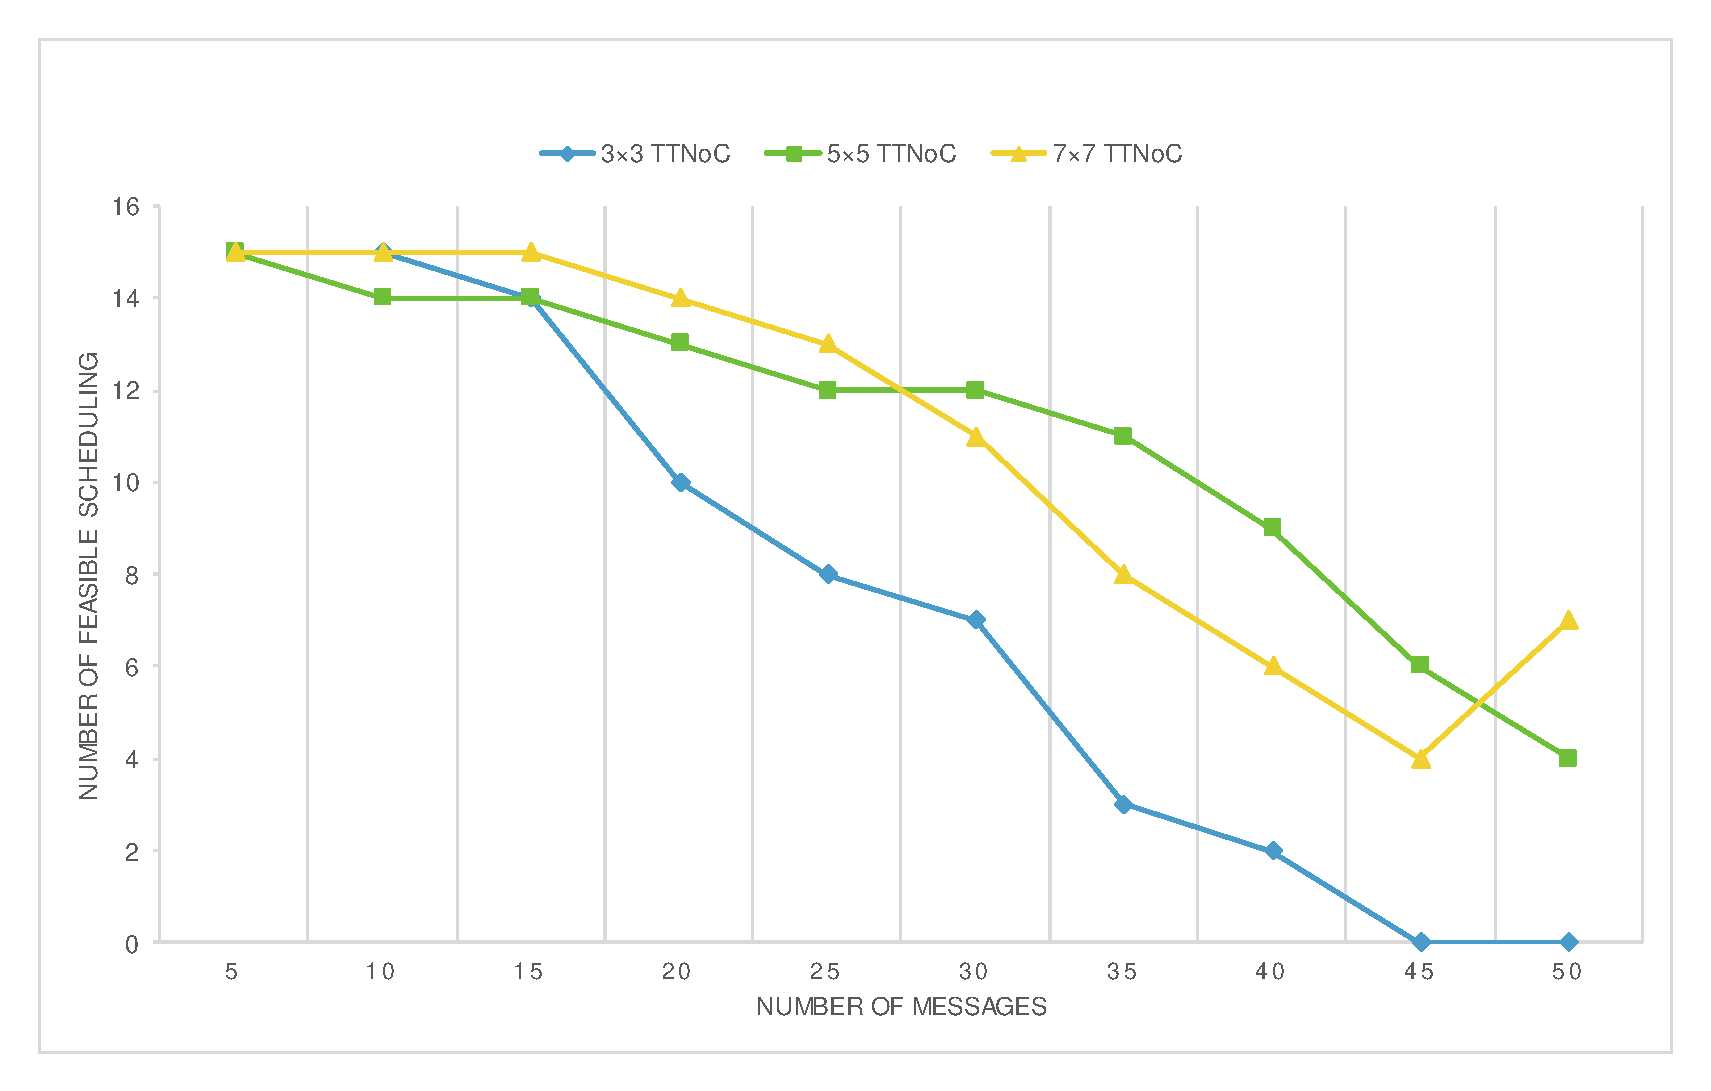
\includegraphics[width=3in]{picture/feasible_case}
	\caption{The number of feasible cases in different test cases}
	\label{f:feasible}
\end{figure}

\subsection{Discussions}

Synthesizing a feasible scheduling depends on the number of messages and the scale of TTNoC.
It is hard for the MA to synthesize a feasible scheduling when the set of messages is large and/or the TTNoC architecture is small.
However,
 except two reason above,
  the mapping between messages and nodes as well as routing strategy also affect generating a feasible solution.
The designer can manually change the map allocation or the routing strategy to the failed scheduling,
 and even design a larger network architecture if needed.
After these changes,
   the feasible scheduling can be generated by the MA iteratively. 

\section{Conclusions \label{s:conclud}}

This paper introduces a memetic algorithm to resolve the scheduling problem of messages on the TTNoC.
We present our memetic algorithm and evaluate with various random generated messages on varying scales of mesh-based TTNoC.
The results of simulation shows that our memetic algorithm is efficient to synthesize a scheduling with less rate of failed scheduling messages, which is about 30\% compared with the synthesis of GA.

In our future work,
the mapping between messages and nodes and routing strategy may be integrated to our consideration before scheduling of messages on the TTNoC.
And the different TTNoC architecture,
i.e. torus, hypercube,
and different local search strategy can be also implemented in our evaluations.




% conference papers do not normally have an appendix


% use section* for acknowledgment
%\section*{Acknowledgment}
%The authors would like to thank...





% trigger a \newpage just before the given reference
% number - used to balance the columns on the last page
% adjust value as needed - may need to be readjusted if
% the document is modified later
%\IEEEtriggeratref{8}
% The "triggered" command can be changed if desired:
%\IEEEtriggercmd{\enlargethispage{-5in}}

% references section

% can use a bibliography generated by BibTeX as a .bbl file
% BibTeX documentation can be easily obtained at:
% http://mirror.ctan.org/biblio/bibtex/contrib/doc/
% The IEEEtran BibTeX style support page is at:
% http://www.michaelshell.org/tex/ieeetran/bibtex/
%\bibliographystyle{IEEEtran}
% argument is your BibTeX string definitions and bibliography database(s)
%\bibliography{IEEEabrv,../bib/paper}
%
% <OR> manually copy in the resultant .bbl file
% set second argument of \begin to the number of references
% (used to reserve space for the reference number labels box)
%% \begin{thebibliography}{1}

%% \bibitem{IEEEhowto:kopka}
%% H.~Kopka and P.~W. Daly, \emph{A Guide to \LaTeX}, 3rd~ed.\hskip 1em plus
%%   0.5em minus 0.4em\relax Harlow, England: Addison-Wesley, 1999.

%% \end{thebibliography}

\bibliographystyle{IEEEtran}
\balance
\bibliography{main}


% that's all folks
\end{document}


